\documentclass[10pt,UKenglish, leqno, xcolor = dvipsnames]{beamer}

\usetheme{UiB}

% Font choice:
\usefonttheme{default}

\usepackage{cite}
\usepackage{amsmath, amsthm, mathtools, color, setspace}
\usepackage{fancyhdr, braket, etoolbox,booktabs,multirow}
\usepackage{xfrac, lmodern, ifsym, bm, multicol, booktabs, pdflscape}
\usepackage[utf8]{inputenx} % For æ, ø, å
\usepackage{csquotes}       % Quotation marks
\usepackage{microtype}      % Improved typography
\usepackage{amssymb}        % Mathematical symbols
\usepackage{mathtools,physics,centernot,tensor}      % Mathematical symbols
\usepackage[absolute, overlay]{textpos} % Arbitrary placement
\setlength{\TPHorizModule}{\paperwidth} % Textpos units
\setlength{\TPVertModule}{\paperheight} % Textpos units
\usepackage[dvipsnames]{xcolor}
\usepackage{tikz}
\usetikzlibrary{tikzmark,calc,overlay-beamer-styles,arrows,shapes}  % Overlay effects for TikZ
\newenvironment{proenv}{\only{\setbeamercolor{local structure}{fg=RoyalBlue}}}{}
\newenvironment{conenv}{\only{\setbeamercolor{local structure}{fg=Maroon}}}{}
\newenvironment{bibbianoenv}{\only{\setbeamercolor{local structure}{fg=Green}}}{}
\DeclarePairedDelimiter{\insieme}{\{}{\}}
\newcommand{\numberset}{\mathbb}
\newcommand{\alg}{\mathfrak}
\newcommand{\Z}{\numberset{Z}}
\newcommand{\R}{\numberset{R}}
\newcommand{\N}{\numberset{N}}
\newcommand{\C}{\numberset{C}}
\newcommand{\A}{\alpha}




\author{Pietro Daniele}
\title{Thesis progress}


\begin{document}
	\tikzstyle{na} = [baseline=-.5ex]
	\tikzstyle{every picture}+=[remember picture]
	
	\begin{frame}{Index}
		\tableofcontents
	\end{frame}

	\begin{frame}{GitHub}
		\vfill
		\begin{center}
			The whole code is available at this GitHib \href{https://github.com/pietrodaniele/thesis}{link}
		\end{center}	
		\vfill
	\end{frame}
	
	%%%%%%%%% 1° week %%%%%%%%%
	\section{1° week}
	\SectionPage
	
		\begin{frame}{Uploading file .root}
			\vfill
			The file uploaded are:
			\begin{itemize}
				\item PowhegPy8\_NNLOPS\_ggH110.root;
				\item PowhegPy8\_NNLOPS\_ggH125.root;
				\item PowhegPy8\_NNLOPS\_ggH130.root;
				\item PowhegPy8\_NNLOPS\_ggH140.root;
			\end{itemize}
			\vfill
		\end{frame}
	
		\begin{frame}{Data}
			\vfill
			\begin{textblock}{5}(0.028,0.35)
				In each file, there is a \texttt{TTree myCatNtuple},\\ which contains all the variables. Only three\\ of them were used:
				\begin{itemize}
					\item \textbf{m\_yy}: mass distribution;
					\item \textbf{EventWeight}: it contains all type of \\weights.
					\item \textbf{cutFlow}
				\end{itemize}
			\end{textblock}
			\begin{textblock}{1}(0.6,0.12)
				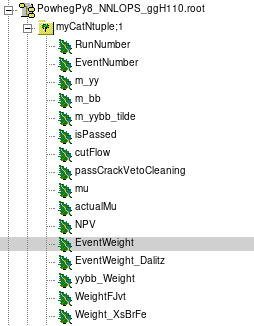
\includegraphics[width=.4\textwidth]{Images/ttre.png}
			\end{textblock}
		\end{frame}
	
		\begin{frame}{$m_{\gamma\gamma}$ distibution}
			\vfill
			Using all entries the distributions at different masses are:
			\includegraphics[width=1.\textwidth]{../Code/Examples/Plots/myy_dist.pdf}
			\vfill
		\end{frame}

		\begin{frame}{Data analysis and fits}
			\vfill
			The distributions are fitted using two type of fit:
			\begin{itemize}
				\item \textbf{gaussian fit}: there are 2 parameters:
				\begin{itemize}
					\item mean $\mu$;
					\item sigma $\sigma$;
				\end{itemize}
				$$
				f(x,\mu,\sigma)= \frac{1}{\sqrt{2\pi\sigma^2}}e^{-\frac{(x-\mu)^2}{2\sigma^2}}
				$$
				\item \textbf{DCB fit}: there are six parameters:
				\begin{itemize}
					\item mean $\mu$;
					\item sigma $\sigma$
					\item a$_1$;
					\item p$_1$;
					\item a$_2$;
					\item p$_2$;
				\end{itemize}
				$$
				f(x,\mu,\sigma,a_1,p_1,a_2,p_2) = \cdots
				$$
			\end{itemize}
			\vfill
		\end{frame}
	
		\begin{frame}{Gaussian and DCB fits}
			\vfill
			Applying the fits to all entries:
			\includegraphics[width=1.\textwidth]{../Code/Examples/Plots/myy+fit.pdf}
			\vfill
		\end{frame}
	
		\begin{frame}{CutFlow}
			\vfill
			Events with at least two isolated $\gamma$ with tight identification could be selected, where the transverse momentum of the leading photon is such that $p_T/m_{\gamma\gamma} > 0.35$, whereas that of the sub-leading photon is $p_T/m_{\gamma\gamma} > 0.25$. Then there are also other demands on the "quality" of data collection and triggers.
			
			\vspace{0.5cm}
			$\Longrightarrow$ Using the \texttt{cutFlow} greater than 13, the events are selected.
			\vfill
		\end{frame}
	
		\begin{frame}{m$_{\gamma\gamma}$ distribution with cutFlow > 13}
			\vfill
			Using \texttt{cutFlow}>13 entries the distributions at different masses are:
			\includegraphics[width=1.\textwidth]{../Code/Examples/Plots/myy_dist_cutFlow.pdf}
			\vfill
		\end{frame}
	
		\begin{frame}{Gaussian and DCB fits with cutFlow > 13}
			\vfill
			Applying the fits to all entries:
			\includegraphics[width=1.\textwidth]{../Code/Examples/Plots/myy+fit_cutFlow.pdf}
			\vfill
		\end{frame}
	
		\begin{frame}{DCB fit and ratio plot [110 GeV]}
			\vfill
			The \texttt{ratio plot} between the fit and the distribution is added to each DCB fit. Using the 110 GeV mass distribution:
			\includegraphics[width=1.\textwidth]{../Code/Examples/Plots/myy_110GeV_DCBfit.pdf}
			\vfill
		\end{frame}
	
		\begin{frame}{DCB fit and ratio plot [125 GeV]}
			\vfill
			The \texttt{ratio plot} between the fit and the distribution is added to each DCB fit. Using the 125 GeV mass distribution:
			\includegraphics[width=1.\textwidth]{../Code/Examples/Plots/myy_125GeV_DCBfit.pdf}
			\vfill
		\end{frame}
	
		\begin{frame}{DCB fit and ratio plot [130 GeV]}
			\vfill
			The \texttt{ratio plot} between the fit and the distribution is added to each DCB fit. Using the 130 GeV mass distribution:
			\includegraphics[width=1.\textwidth]{../Code/Examples/Plots/myy_130GeV_DCBfit.pdf}
			\vfill
		\end{frame}
	
		\begin{frame}{DCB fit and ratio plot [140 GeV]}
			\vfill
			The \texttt{ratio plot} between the fit and the distribution is added to each DCB fit. Using the 140 GeV mass distribution:
			\includegraphics[width=1.\textwidth]{../Code/Examples/Plots/myy_140GeV_DCBfit.pdf}
			\vfill
		\end{frame}
	
		\begin{frame}{DCB fit+ratioplot [110 GeV] (cutFlow > 13)}
			\vfill
			The \texttt{ratio plot} between the fit and the distribution is added to each DCB fit. Using the 110 GeV mass distribution with \texttt{cutFlow} > 13:
			\includegraphics[width=1.\textwidth]{../Code/Examples/Plots/myy_110GeV_DCBfit_cutFlow.pdf}
			\vfill
		\end{frame}
		
		\begin{frame}{DCB fit+ratioplot [125 GeV] (cutFlow > 13)}
			\vfill
			The \texttt{ratio plot} between the fit and the distribution is added to each DCB fit. Using the 125 GeV mass distribution with \texttt{cutFlow} > 13:
			\includegraphics[width=1.\textwidth]{../Code/Examples/Plots/myy_125GeV_DCBfit_cutFlow.pdf}
			\vfill
		\end{frame}
		
		\begin{frame}{DCB fit+ratioplot [130 GeV] (cutFlow > 13)}
			\vfill
			The \texttt{ratio plot} between the fit and the distribution is added to each DCB fit. Using the 130 GeV mass distribution with \texttt{cutFlow} > 13:
			\includegraphics[width=1.\textwidth]{../Code/Examples/Plots/myy_130GeV_DCBfit_cutFlow.pdf}
			\vfill
		\end{frame}
		
		\begin{frame}{DCB fit+ratioplot [140 GeV] (cutFlow > 13)}
			\vfill
			The \texttt{ratio plot} between the fit and the distribution is added to each DCB fit. Using the 140 GeV mass distribution with \texttt{cutFlow} > 13:
			\includegraphics[width=1.\textwidth]{../Code/Examples/Plots/myy_140GeV_DCBfit_cutFlow.pdf}
			\vfill
		\end{frame}
	
	%%%%%%%%% 2° week %%%%%%%%%
	\section{2° week}
	\SectionPage
	
		\begin{frame}{DSCB(m$_{h}$)}
			\vfill
			The DSCD fit are studied with 3 different methods, in addiction to all free parameters fit:
			\begin{enumerate}
				\item multi-fit;
				\item $\mu$ and $\sigma$ are functions of $m_h$;
				\item all parameters are functions of $m_h$;
			\end{enumerate}
			\vfill
		\end{frame}

		\begin{frame}{DSCB multifit}
			\vfill
			A DSCB multifit consists of a series of consecutive fits:
			\begin{enumerate}
				\item fit on $\mu$ and $\sigma$, tails params fixed;
				\item fit on tails params, $\mu$ and $\sigma$ fixed;
				\item fit on all parameters;
			\end{enumerate}
			\vfill
		\end{frame}
	
		\begin{frame}{DSCB multifit [110 GeV]}
			\vfill
			\includegraphics[width=1.\textwidth]{../Code/Examples/Plots/myy_110GeV_DCBfit_cutFlow_multifit.pdf}
			\vfill
		\end{frame}
	
		\begin{frame}{DSCB multifit [125 GeV]}
			\vfill
			\includegraphics[width=1.\textwidth]{../Code/Examples/Plots/myy_125GeV_DCBfit_cutFlow_multifit.pdf}
			\vfill
		\end{frame}
	
		\begin{frame}{DSCB multifit [130 GeV]}
			\vfill
			\includegraphics[width=1.\textwidth]{../Code/Examples/Plots/myy_130GeV_DCBfit_cutFlow_multifit.pdf}
			\vfill
		\end{frame}
	
		\begin{frame}{DSCB multifit [140 GeV]}
			\vfill
			\includegraphics[width=1.\textwidth]{../Code/Examples/Plots/myy_140GeV_DCBfit_cutFlow_multifit.pdf}
			\vfill
		\end{frame}
	
		\begin{frame}{$\mu(m_h)$}
			\vfill
			Fitting the $\mu$ values at different $m_h$ with a linear fit:
			$$
			\mu(m_h)=A+B\cdot m_h
			$$
			\centering
			\includegraphics[width=.72\textwidth]{../Code/Examples/Plots/mu_fit.pdf}
			\vfill
		\end{frame}
	
		\begin{frame}{$\sigma(m_h)$}
			\vfill
			Fitting the $\sigma$ values at different $m_h$ with a linear fit:
			$$
			\sigma(m_h)=A+B\cdot m_h
			$$
			\centering
			\includegraphics[width=.72\textwidth]{../Code/Examples/Plots/sigma_fit.pdf}
			\vfill
		\end{frame}
	
		\begin{frame}{$a_1(m_h)$}
			\vfill
			Fitting the $a_1$ values at different $m_h$ with a linear fit:
			$$
			a_1(m_h)=A+B\cdot m_h
			$$
			\centering
			\includegraphics[width=.72\textwidth]{../Code/Examples/Plots/a1_fit.pdf}
			\vfill
		\end{frame}
	
		\begin{frame}{$p_1(m_h)$}
			\vfill
			Fitting the $p_1$ values at different $m_h$ with a linear fit:
			$$
			p_1(m_h)=A+B\cdot m_h
			$$
			\centering
			\includegraphics[width=.72\textwidth]{../Code/Examples/Plots/p1_fit.pdf}
			\vfill
		\end{frame}
	
		\begin{frame}{$a_2(m_h)$}
			\vfill
			Fitting the $a_2$ values at different $m_h$ with a linear fit:
			$$
			a_2(m_h)=A+B\cdot m_h
			$$
			\centering
			\includegraphics[width=.72\textwidth]{../Code/Examples/Plots/a2_fit.pdf}
			\vfill
		\end{frame}
	
		\begin{frame}{$p_2(m_h)$}
			\vfill
			Fitting the $p_2$ values at different $m_h$ with a linear fit:
			$$
			p_2(m_h)=A+B\cdot m_h
			$$
			\centering
			\includegraphics[width=.72\textwidth]{../Code/Examples/Plots/p2_fit.pdf}
			\vfill
		\end{frame}
	
		\begin{frame}{DSCB(m$_{h}$) with $\mu(m_h)$ and $\sigma(m_h)$ [110 GeV]}
			\vfill
			\includegraphics[width=1.\textwidth]{../Code/Examples/Plots/myy_110GeV_DCBfit_cutFlow_mu_sigma_mh.pdf}
			\vfill
		\end{frame}
	
		\begin{frame}{DSCB(m$_{h}$) with $\mu(m_h)$ and $\sigma(m_h)$ [125 GeV]}
			\vfill
			\includegraphics[width=1.\textwidth]{../Code/Examples/Plots/myy_125GeV_DCBfit_cutFlow_mu_sigma_mh.pdf}
			\vfill
		\end{frame}

		\begin{frame}{DSCB(m$_{h}$) with $\mu(m_h)$ and $\sigma(m_h)$ [130 GeV]}
			\vfill
			\includegraphics[width=1.\textwidth]{../Code/Examples/Plots/myy_130GeV_DCBfit_cutFlow_mu_sigma_mh.pdf}
			\vfill
		\end{frame}	
	
		\begin{frame}{DSCB(m$_{h}$) with $\mu(m_h)$ and $\sigma(m_h)$ [140 GeV]}
			\vfill
			\includegraphics[width=1.\textwidth]{../Code/Examples/Plots/myy_140GeV_DCBfit_cutFlow_mu_sigma_mh.pdf}
			\vfill
		\end{frame}
	
		\begin{frame}{DSCB(m$_{h}$) with all params$(m_h)$ [110 GeV]}
			\vfill
			\includegraphics[width=1.\textwidth]{../Code/Examples/Plots/myy_110GeV_DCBfit_cutFlow_all_mh.pdf}
			\vfill
		\end{frame}
	
		\begin{frame}{DSCB(m$_{h}$) with all params$(m_h)$ [125 GeV]}
			\vfill
			\includegraphics[width=1.\textwidth]{../Code/Examples/Plots/myy_125GeV_DCBfit_cutFlow_all_mh.pdf}
			\vfill
		\end{frame}
	
		\begin{frame}{DSCB(m$_{h}$) with all params$(m_h)$ [130 GeV]}
			\vfill
			\includegraphics[width=1.\textwidth]{../Code/Examples/Plots/myy_130GeV_DCBfit_cutFlow_all_mh.pdf}
			\vfill
		\end{frame}
	
		\begin{frame}{DSCB(m$_{h}$) with all params$(m_h)$ [140 GeV]}
			\vfill
			\includegraphics[width=1.\textwidth]{../Code/Examples/Plots/myy_140GeV_DCBfit_cutFlow_all_mh.pdf}
			\vfill
		\end{frame}
	
		\begin{frame}{Global fit [110 GeV]}
			\vfill
			\includegraphics[width=1.\textwidth]{../Code/Examples/Plots/myy_110GeV_DCBfit_cutFlow_global.pdf}
			\vfill
		\end{frame}
	
		\begin{frame}{Global fit [125 GeV]}
			\vfill
			\includegraphics[width=1.\textwidth]{../Code/Examples/Plots/myy_125GeV_DCBfit_cutFlow_global.pdf}
			\vfill
		\end{frame}
	
		\begin{frame}{Global fit [130 GeV]}
			\vfill
			\includegraphics[width=1.\textwidth]{../Code/Examples/Plots/myy_130GeV_DCBfit_cutFlow_global.pdf}
			\vfill
		\end{frame}
	
		\begin{frame}{Global fit [140 GeV]}
			\vfill
			\includegraphics[width=1.\textwidth]{../Code/Examples/Plots/myy_140GeV_DCBfit_cutFlow_global.pdf}
			\vfill
		\end{frame}
		
		\begin{frame}{Single vs Global fit params: $\mu$}
			\vfill
			\includegraphics[width=1.\textwidth]{../Code/Examples/Plots/mu_param.pdf}
			\vfill
		\end{frame}

		\begin{frame}{Single vs Global fit params: $\sigma$}
			\vfill
			\includegraphics[width=1.\textwidth]{../Code/Examples/Plots/width_param.pdf}
			\vfill
		\end{frame}
		
		\begin{frame}{Single vs Global fit params: $a_1$}
			\vfill
			\includegraphics[width=1.\textwidth]{../Code/Examples/Plots/a1_param.pdf}
			\vfill
		\end{frame}
	
		\begin{frame}{Single vs Global fit params: $p_1$}
			\vfill
			\includegraphics[width=1.\textwidth]{../Code/Examples/Plots/p1_param.pdf}
			\vfill
		\end{frame}
	
		\begin{frame}{Single vs Global fit params: $a_2$}
			\vfill
			\includegraphics[width=1.\textwidth]{../Code/Examples/Plots/a2_param.pdf}
			\vfill
		\end{frame}
	
		\begin{frame}{Single vs Global fit params: $p_2$}
			\vfill
			\includegraphics[width=1.\textwidth]{../Code/Examples/Plots/p2_param.pdf}
			\vfill
		\end{frame}
	
		\begin{frame}{Efficiencies($m_h$)}
			\vspace{.8cm}
			\centering
			$eff = \frac{\#\ of\ events\ with\ cutFlow>13}{\#\ of\ all\ events}$
			\vspace{2.5cm}
			\includegraphics[width=.85\textwidth]{../Code/Examples/Plots/efficiencies.pdf}
		\end{frame}
	
	%%%%%%%%% 3° week %%%%%%%%%
	\section{3° week}
	\SectionPage
	
		\begin{frame}{3° week assignments}
			\vfill
			\begin{itemize}
				\item fix the X-axis:" $m_{yy}\ [GeV]$" to "$m_{h}\ [GeV]$";
				\item create a fit with all parameters as function of $m_H$;
				\item fit without a dataset:
				\begin{itemize}
					\item the fit is build using 110, 130, 140 GeV datasets;
					\item once the is created, it is applied to the 125 dataset.
				\end{itemize}
				\item add errors bars;
				\item background MC:
				\begin{itemize}
					\item plot the mass distribution;
					\item apply a exp fit.
				\end{itemize}
				\item build a p$_{0}$ scan on MC;
			\end{itemize}
			\vfill
		\end{frame}
	
		\begin{frame}{Global fit all params($m_H$) [110 GeV]}
			\vfill
			\includegraphics[width=1.\textwidth]{../Code/Examples/Plots/myy_110GeV_DCBfit_cutFlow_global_all.pdf}
			\vfill
		\end{frame}
	
		\begin{frame}{Global fit all params($m_H$) [125 GeV]}
			\vfill
			\includegraphics[width=1.\textwidth]{../Code/Examples/Plots/myy_125GeV_DCBfit_cutFlow_global_all.pdf}
			\vfill
		\end{frame}
	
		\begin{frame}{Global fit all params($m_H$) [130 GeV]}
			\vfill
			\includegraphics[width=1.\textwidth]{../Code/Examples/Plots/myy_130GeV_DCBfit_cutFlow_global_all.pdf}
			\vfill
		\end{frame}
	
		\begin{frame}{Global fit all params($m_H$) [140 GeV]}
			\vfill
			\includegraphics[width=1.\textwidth]{../Code/Examples/Plots/myy_140GeV_DCBfit_cutFlow_global_all.pdf}
			\vfill
		\end{frame}
		
		\begin{frame}{Single vs Global fit params: $\mu(m_h)$}
			\vfill
			\includegraphics[width=1.\textwidth]{../Code/Examples/Plots/mu_param_all.pdf}
			\vfill
		\end{frame}
		
		\begin{frame}{Single vs Global fit params: $\sigma(m_h)$}
			\vfill
			\includegraphics[width=1.\textwidth]{../Code/Examples/Plots/width_param_all.pdf}
			\vfill
		\end{frame}
		
		\begin{frame}{Single vs Global fit params: $a_1(m_h)$}
			\vfill
			\includegraphics[width=1.\textwidth]{../Code/Examples/Plots/a1_param_all.pdf}
			\vfill
		\end{frame}
		
		\begin{frame}{Single vs Global fit params: $p_1(m_h)$}
			\vfill
			\includegraphics[width=1.\textwidth]{../Code/Examples/Plots/p1_param_all.pdf}
			\vfill
		\end{frame}
		
		\begin{frame}{Single vs Global fit params: $a_2(m_h)$}
			\vfill
			\includegraphics[width=1.\textwidth]{../Code/Examples/Plots/a2_param_all.pdf}
			\vfill
		\end{frame}
		
		\begin{frame}{Single vs Global fit params: $p_2(m_h)$}
			\vfill
			\includegraphics[width=1.\textwidth]{../Code/Examples/Plots/p2_param_all.pdf}
			\vfill
/Code		\end{frame}
	
		\begin{frame}{Global fit($m_H$) (no 125) [110 GeV]}
			\vfill
			\includegraphics[width=1.\textwidth]{../Code/Examples/Plots/myy_110GeV_DCBfit_cutFlow_no125.pdf}
			\vfill
		\end{frame}
		
		\begin{frame}{Global fit($m_H$) (no 125) [130 GeV]}
			\vfill
			\includegraphics[width=1.\textwidth]{../Code/Examples/Plots/myy_130GeV_DCBfit_cutFlow_no125.pdf}
			\vfill
		\end{frame}
		
		\begin{frame}{Global fit($m_H$) (no 125) [140 GeV]}
			\vfill
			\includegraphics[width=1.\textwidth]{../Code/Examples/Plots/myy_140GeV_DCBfit_cutFlow_no125.pdf}
			\vfill
		\end{frame}
	
		\begin{frame}{Fit without 125 GeV dataset}
			\vfill
			\includegraphics[width=1.\textwidth]{../Code/Examples/Plots/myy_125GeV_DCBfit_cutFlow_no125.pdf}
			\vfill 
		\end{frame}
	
		\begin{frame}{Background MC}
			\vfill
			\includegraphics[width=1.\textwidth]{../Code/Examples/Plots/backgroundMC_dist.pdf}
			\vfill 
		\end{frame}
	
		\begin{frame}{Only background workspace}
			\vfill
			Simultaneous fit composed by 4 DSCB (signal) + exp fit (background). Only background dataset.
			\begin{center}
				\includegraphics[width=.9\textwidth]{../Code/Examples/Plots/only_bkg_plot.pdf}
			\end{center}
			\vfill
		\end{frame}
	
		\begin{frame}{Signal+background workspace [140 GeV]}
			\vfill
			Simultaneous fit composed by 4 DSCB (signal) + exp fit (background). Signal+background dataset.
			\begin{center}
				\includegraphics[width=.9\textwidth]{../Code/Examples/Plots/sig_bkg_plot_140GeV.pdf}
			\end{center}
			\vfill
		\end{frame}
	
		\begin{frame}{Signal+background workspace [130 GeV]}
			\vfill
			Simultaneous fit composed by 4 DSCB (signal) + exp fit (background). Signal+background dataset.
			\begin{center}
				\includegraphics[width=.9\textwidth]{../Code/Examples/Plots/sig_bkg_plot_130GeV.pdf}
			\end{center}
			\vfill
		\end{frame}

		\begin{frame}{Signal+background workspace [125 GeV]}
			\vfill
			Simultaneous fit composed by 4 DSCB (signal) + exp fit (background). Signal+background dataset.
			\begin{center}
				\includegraphics[width=.9\textwidth]{../Code/Examples/Plots/sig_bkg_plot_125GeV.pdf}
			\end{center}
			\vfill
		\end{frame}
	
	%%%%%%%%% 4° week %%%%%%%%%
	\section{4° week}
	\SectionPage
	
		\begin{frame}{4° week assignments}
			\vfill
			\begin{itemize}
				\item chiSquare check;
				\item single and global fit comparison:
				\begin{itemize}
					\item plot with chiSquare;
					\item y-log plot with chiSquare; 
				\end{itemize}
				\item normalisation check;
				\item efficiency check;
				\item only bkg and sig+bkg models study:
				\begin{itemize}
					\item m$_{\gamma\gamma}$ distribution analysis;
					\item p$_0$ scan;
					\item CLs limit analysis;
				\end{itemize}
			\end{itemize}
			\vfill
		\end{frame}
	
		\begin{frame}{ChiSquare}
			\vfill
			\centering
			\texttt{frame->chiSquare("Fit","Data")}
			\includegraphics[width=1.\textwidth]{../Code/Examples/Plots/chiSquare.png}
			\vfill
		\end{frame}
	
		\begin{frame}{Single vs global fit comp. [110 Gev]}
			\vfill
			\includegraphics[width=1.\textwidth]{../Code/Examples/Plots/comp_plot_110GeV.pdf}
			\vfill
		\end{frame}
	
		\begin{frame}{Single vs global fit comp. [110 Gev] (ylog)}
			\vfill
			\includegraphics[width=1.\textwidth]{../Code/Examples/Plots/comp_plot_110GeV_log.pdf}
			\vfill
		\end{frame}
	
		\begin{frame}{Single vs global fit comp. [125 Gev]}
			\vfill
			\includegraphics[width=1.\textwidth]{../Code/Examples/Plots/comp_plot_125GeV.pdf}
			\vfill
		\end{frame}
		
		\begin{frame}{Single vs global fit comp. [125 Gev] (ylog)}
			\vfill
			\includegraphics[width=1.\textwidth]{../Code/Examples/Plots/comp_plot_125GeV_log.pdf}
			\vfill
		\end{frame}
	
		\begin{frame}{Single vs global fit comp. [130 Gev]}
			\vfill
			\includegraphics[width=1.\textwidth]{../Code/Examples/Plots/comp_plot_130GeV.pdf}
			\vfill
		\end{frame}
		
		\begin{frame}{Single vs global fit comp. [130 Gev] (ylog)}
			\vfill
			\includegraphics[width=1.\textwidth]{../Code/Examples/Plots/comp_plot_130GeV_log.pdf}
			\vfill
		\end{frame}
	
		\begin{frame}{Single vs global fit comp. [140 Gev]}
			\vfill
			\includegraphics[width=1.\textwidth]{../Code/Examples/Plots/comp_plot_140GeV.pdf}
			\vfill
		\end{frame}
		
		\begin{frame}{Single vs global fit comp. [140 Gev] (ylog)}
			\vfill
			\includegraphics[width=1.\textwidth]{../Code/Examples/Plots/comp_plot_140GeV_log.pdf}
			\vfill
		\end{frame}
	
		\begin{frame}{Check normalisations}
			\vfill
			\centering
			My and Elena's results are compared in:
			\href{https://docs.google.com/spreadsheets/d/1HAke9uer_arNKmDrZkEBPS_DiHJFm9zSdsW57HAgCL4/edit?usp=sharing}{docs}
			\vfill
		\end{frame}
	
		\begin{frame}{Efficiencies($m_h$)}
			\vspace{.5cm}
			\begin{center}
				$eff = \sum\frac{weight\ of\ event\ with\ cutFlow>13}{Weight_{XsBrFe}}$
			\end{center}
			\vspace{.5cm}
			\begin{center}
				\includegraphics[width=.8\textwidth]{../Code/Examples/Plots/efficiencies.pdf}
			\end{center}
		\end{frame}
	
		\begin{frame}{Only background}
			\vfill
			\includegraphics[width=1.\textwidth]{../Code/Examples/Plots/only_bkg_plot.pdf}
			\vfill
		\end{frame}
	
		\begin{frame}{Only background p0 scan}
			\vfill
			\includegraphics[width=1.\textwidth]{../Code/Examples/Plots/p0_plot_only_bkg.pdf}
			\vfill
		\end{frame}
	
		\begin{frame}{Only background limit}
			\vfill
			\includegraphics[width=1.\textwidth]{../Code/Examples/Plots/limit_plot_only_bkg.pdf}
			\vfill
		\end{frame}
	
		\begin{frame}{Sig+bkg [110 GeV]}
			\vfill
			\includegraphics[width=1.\textwidth]{../Code/Examples/Plots/sig_bkg_plot_110GeV.pdf}
			\vfill
		\end{frame}
	
		\begin{frame}{Sig+bkg p0 scan [110 GeV]}
			\vfill
			\includegraphics[width=1.\textwidth]{../Code/Examples/Plots/p0_plot_110GeV.pdf}
			\vfill
		\end{frame}
		
		\begin{frame}{Sig+bkg limit [110 GeV]}
			\vfill
			\includegraphics[width=1.\textwidth]{../Code/Examples/Plots/limit_plot_110GeV.pdf}
			\vfill
		\end{frame}
	
		\begin{frame}{Sig+bkg [125 GeV]}
			\vfill
			\includegraphics[width=1.\textwidth]{../Code/Examples/Plots/sig_bkg_plot_125GeV.pdf}
			\vfill
		\end{frame}
		
		\begin{frame}{Sig+bkg p0 scan [125 GeV]}
			\vfill
			\includegraphics[width=1.\textwidth]{../Code/Examples/Plots/p0_plot_125GeV.pdf}
			\vfill
		\end{frame}
		
		\begin{frame}{Sig+bkg limit scan [125 GeV]}
			\vfill
			\includegraphics[width=1.\textwidth]{../Code/Examples/Plots/limit_plot_125GeV.pdf}
			\vfill
		\end{frame}
		
		\begin{frame}{Sig+bkg [130 GeV]}
			\vfill
			\includegraphics[width=1.\textwidth]{../Code/Examples/Plots/sig_bkg_plot_130GeV.pdf}
			\vfill
		\end{frame}
		
		\begin{frame}{Sig+bkg p0 scan [130 GeV]}
			\vfill
			\includegraphics[width=1.\textwidth]{../Code/Examples/Plots/p0_plot_130GeV.pdf}
			\vfill
		\end{frame}
		
		\begin{frame}{Sig+bkg limit scan [130 GeV]}
			\vfill
			\includegraphics[width=1.\textwidth]{../Code/Examples/Plots/limit_plot_130GeV.pdf}
			\vfill
		\end{frame}
	
		\begin{frame}{Sig+bkg [140 GeV]}
			\vfill
			\includegraphics[width=1.\textwidth]{../Code/Examples/Plots/sig_bkg_plot_140GeV.pdf}
			\vfill
		\end{frame}
		
		\begin{frame}{Sig+bkg p0 scan [140 GeV]}
			\vfill
			\includegraphics[width=1.\textwidth]{../Code/Examples/Plots/p0_plot_140GeV.pdf}
			\vfill
		\end{frame}
		
		\begin{frame}{Sig+bkg limit scan [140 GeV]}
			\vfill
			\includegraphics[width=1.\textwidth]{../Code/Examples/Plots/limit_plot_140GeV.pdf}
			\vfill
		\end{frame}
	
	%%%%%%%%% 5° week %%%%%%%%%
	\section{5° week}
	\SectionPage
		
		\begin{frame}{Efficiencies(m$_H$) fit}
			\vfill
			\includegraphics[width=1.\textwidth]{../images/efficiencies_fit.pdf}
			\vfill
		\end{frame}
	
		\begin{frame}{Yields(m$_H$) fit}
			\vfill
			\includegraphics[width=1.\textwidth]{../images/yields_fit.pdf}
			\vfill
		\end{frame}
	
		\begin{frame}{Workspace}
			\vfill
			\includegraphics[width=1.\textwidth]{../images/ggHyy_rebin10.pdf}
			\vfill
		\end{frame}
	
		\begin{frame}{AsimovDataset $\mu=0$}
			\vfill
			\includegraphics[width=1.\textwidth]{../images/plot_AsimovData_0_ggHyy.pdf}
			\vfill
		\end{frame}
	
		\begin{frame}{AsimovDataset $\mu=1$ and $m_H=125$}
			\vfill
			\includegraphics[width=1.\textwidth]{../images/plot_AsimovData_1_125_ggHyy.pdf}
			\vfill
		\end{frame}
	
	%%%%%%%%% 6° week %%%%%%%%%
	\section{6° week}
	\SectionPage
		
		\begin{frame}{Efficiencies(m$_H$) fit}
			\vfill
			\includegraphics[width=1.\textwidth]{../images/efficiencies_fit_1.pdf}
			\vfill
		\end{frame}
	
		\begin{frame}{X-Section(mH)}
			x-section values --> \href{https://twiki.cern.ch/twiki/bin/view/LHCPhysics/CERNYellowReportPageBSMAt13TeV}{link}. Errors are evaluated using QCD and (Pdf+$\alpha$) \% errors (Quadratic sum).
			\vfill
			\centering
			\includegraphics[width=.9\textwidth]{../images/x_section_fit.pdf}
			\vfill
		\end{frame}
	
		\begin{frame}{Branching Fraction(mH)}
			br values --> \href{https://arxiv.org/abs/1307.1347}{link}. 
			\vfill
			\centering
			\includegraphics[width=.9\textwidth]{../images/br_fit_1.pdf}
			\vfill
		\end{frame}
	
		\begin{frame}{Workspace}
			\vfill
			\includegraphics[width=1.\textwidth]{../images/ggHyy_efxsbr.pdf}
			\vfill
		\end{frame}
	
	%%%%%%%%% 7° week %%%%%%%%%
	\section{7° week}
	\SectionPage
	
		\begin{frame}{Efficiencies(m$_H$) fit}
			\vfill
			\includegraphics[width=1.\textwidth]{../images/efficiencies_fit_1.pdf}
			\vfill
		\end{frame}
	
		\begin{frame}{X-Section(mH)}
			x-section values --> \href{https://twiki.cern.ch/twiki/bin/view/LHCPhysics/CERNYellowReportPageBSMAt13TeV}{link}. Errors are evaluated using QCD and (Pdf+$\alpha$) \% errors (Quadratic sum).
			\vfill
			\centering
			\includegraphics[width=.9\textwidth]{../images/x_section_fit.pdf}
			\vfill
		\end{frame}
	
		\begin{frame}{Branching Fraction(mH)}
			br values --> \href{https://arxiv.org/abs/1307.1347}{link}. 
			\vfill
			\centering
			\includegraphics[width=1.\textwidth]{../images/br_fit.pdf}
			\vfill
		\end{frame}
	
		\begin{frame}{Check yields(mH)}
			\vfill
			\centering
			$yield(mH) = x\-s(mH) \cdot eff(mH) \cdot br(mH) \cdot LumiRun2$
			\vspace{.5cm}
			\includegraphics[width=.9\textwidth]{../images/check_yields.pdf}
			\vfill
		\end{frame}
	
		\begin{frame}{Workspace ggHyy\_MCpdf}
			\vfill
			\includegraphics[width=1.\textwidth]{../images/ggHyy_MCpdf.pdf}
			\vfill
		\end{frame}
	
		\begin{frame}{AsimovData $\mu$=0, ggHyy\_MCpdf}
			\vfill
			\includegraphics[width=1.\textwidth]{../images/AsimovData_0_ggHyy_MCpdf.pdf}
			\vfill
		\end{frame}
	
		\begin{frame}{AsimovData $\mu(m_H)$, ggHyy\_MCpdf}
			\vfill
			\includegraphics[width=1.\textwidth]{../images/mu_AsimovData_0_ggHyy_MCpdf_plot.pdf}
			\vfill
		\end{frame}
	
		\begin{frame}{AsimovData $\mu$=1, $m_H$=125, ggHyy\_MCpdf}
			\vfill
			\includegraphics[width=1.\textwidth]{../images/AsimovData_1_125_ggHyy_MCpdf.pdf}
			\vfill
		\end{frame}
	
		\begin{frame}{AsimovData $\mu(m_H)$, ggHyy\_MCpdf}
			\vfill
			\includegraphics[width=1.\textwidth]{../images/mu_AsimovData_1_125_ggHyy_MCpdf_plot.pdf}
			\vfill
		\end{frame}
	
		\begin{frame}{AsimovData $\mu$=1, $m_H$=125 + fit, ggHyy\_MCpdf}
			\vfill
			\includegraphics[width=1.\textwidth]{../images/AsimovData_1_125_fit_ggHyy_MCpdf.pdf}
			\vfill
		\end{frame}
	
		\begin{frame}{AsimovData $\mu$=1, $m_H$=125 + fit(mH=110), ggHyy\_MCpdf}
			\vfill
			\includegraphics[width=1.\textwidth]{../images/AsimovData_1_125_check_ggHyy_MCpdf.pdf}
			\vfill
		\end{frame}
	
		\begin{frame}{AsimovData $\mu$=0 limits}
			\vfill
			\includegraphics[width=1.\textwidth]{../images/plot_AsimovData_0_ggHyy_MCpdf.pdf}
			\vfill
		\end{frame}
			
		\begin{frame}{AsimovData $\mu$=1, $m_H$=125 limits}
			\vfill
			\includegraphics[width=1.\textwidth]{../images/plot_AsimovData_1_125_ggHyy_MCpdf.pdf}
			\vfill
		\end{frame}
	
	%%%%%%%%% 8° week %%%%%%%%%
	\section{8° week}
	\SectionPage
	
		\begin{frame}{Background [95,195] GeV}
			\vfill
			I have merged 3 MC ntuple samples in [95,195] GeV:
			\begin{itemize}
				\item Sherpa2\_myy\_50\_90.root;
				\item Sherpa2\_myy\_90\_175.root;
				\item Sherpa2\_myy\_175\_2000.root;
			\end{itemize}
			\vfill
		\end{frame}
	
		\begin{frame}{Background [95,195] GeV plot + bkg\_fit}
			\vfill
			\includegraphics[width=1.\textwidth]{../images/background_95_195GeV_fit.pdf}
			\vfill
		\end{frame}
	
		\begin{frame}{Workspace ggHyy\_MC}
			\vfill
			\includegraphics[width=1.\textwidth]{../images/ggHyy_MC.pdf}
			\vfill
		\end{frame}
		
		\begin{frame}{AsimovData $\mu$=0, ggHyy\_MC}
			\vfill
			\includegraphics[width=1.\textwidth]{../images/AsimovData_0_ggHyy_MC.pdf}
			\vfill
		\end{frame}
		
		\begin{frame}{AsimovData $\mu(m_H)$, ggHyy\_MC}
			\vfill
			\includegraphics[width=1.\textwidth]{../images/mu_AsimovData_0_ggHyy_MC_plot.pdf}
			\vfill
		\end{frame}
		
		\begin{frame}{AsimovData $\mu$=1, $m_H$=125, ggHyy\_MC}
			\vfill
			\includegraphics[width=1.\textwidth]{../images/AsimovData_1_125_ggHyy_MC.pdf}
			\vfill
		\end{frame}
		
		\begin{frame}{AsimovData $\mu(m_H)$, ggHyy\_MC}
			\vfill
			\includegraphics[width=1.\textwidth]{../images/mu_AsimovData_1_125_ggHyy_MC_plot.pdf}
			\vfill
		\end{frame}
		
		\begin{frame}{AsimovData $\mu$=1, $m_H$=125 + fit, ggHyy\_MC}
			\vfill
			\includegraphics[width=1.\textwidth]{../images/AsimovData_1_125_fit_ggHyy_MC.pdf}
			\vfill
		\end{frame}
		
		\begin{frame}{AsimovData $\mu$=1, $m_H$=125 + fit(mH=110), ggHyy\_MC}
			\vfill
			\includegraphics[width=1.\textwidth]{../images/AsimovData_1_125_check_ggHyy_MC.pdf}
			\vfill
		\end{frame}
		
		\begin{frame}{AsimovData $\mu$=0 limits}
			\vfill
			\includegraphics[width=1.\textwidth]{../images/plot_AsimovData_0_ggHyy_MC.pdf}
			\vfill
		\end{frame}
		
		\begin{frame}{AsimovData $\mu$=1, $m_H$=125 limits}
			\vfill
			\includegraphics[width=1.\textwidth]{../images/plot_AsimovData_1_125_ggHyy_MC.pdf}
			\vfill
		\end{frame}
		
	%%%%%%%%% 9° week %%%%%%%%%
	\section{9° week}
	\SectionPage
		
		\begin{frame}{Background [100,195] GeV plot + bkg\_fit}
			\vfill
			\includegraphics[width=1.\textwidth]{../images/week_9/background_100_195GeV_fit.pdf}
			\vfill
		\end{frame}
	
		\begin{frame}{Categories}
			\vfill
			\begin{itemize}
				\item \textbf{unconv}: 2 unconv photons (\texttt{ph*\_Rconv $\epsilon$ ]0,800[ mm})
				\item \textbf{1\_conv}: only 1 conv photon (\texttt{ph*\_Rconv $\epsilon$ (0,800) mm})
				\item \textbf{eta\_1}: 2 phs in the inner eta region (\texttt{|ph*\_eta|<0.75})
				\item \textbf{eta\_2}: at least 1 ph in the trans eta region  (\texttt{1.3<|ph*\_eta|<1.37, 1.52<|ph*\_eta|<1.75})
				\item \textbf{eta\_3}: 2 phs in ext eta region (\texttt{|ph*\_eta|>1.75})
			\end{itemize}
			\vfill
		\end{frame}
	
		\begin{frame}{Categories}
			\vfill
			\includegraphics[width=1.\textwidth]{../images/week_9/category.png}
			\vfill
		\end{frame}
	
		\begin{frame}{Eff unconv eta\_1}
			\vfill
			\includegraphics[width=1.\textwidth]{../images/week_9/efficiencies_fit_unconv_eta_1.pdf}
			\vfill
		\end{frame}
	
		\begin{frame}{Eff unconv eta\_2}
			\vfill
			\includegraphics[width=1.\textwidth]{../images/week_9/efficiencies_fit_unconv_eta_2.pdf}
			\vfill
		\end{frame}
	
		\begin{frame}{Eff unconv eta\_3}
			\vfill
			\includegraphics[width=1.\textwidth]{../images/week_9/efficiencies_fit_unconv_eta_3.pdf}
			\vfill
		\end{frame}
	
		\begin{frame}{Eff 1\_conv eta\_1}
			\vfill
			\includegraphics[width=1.\textwidth]{../images/week_9/efficiencies_fit_1_conv_eta_1.pdf}
			\vfill
		\end{frame}
	
		\begin{frame}{Eff 1\_conv eta\_2}
			\vfill
			\includegraphics[width=1.\textwidth]{../images/week_9/efficiencies_fit_1_conv_eta_2.pdf}
			\vfill
		\end{frame}
	
		\begin{frame}{Eff 1\_conv eta\_3}
			\vfill
			\includegraphics[width=1.\textwidth]{../images/week_9/efficiencies_fit_1_conv_eta_3.pdf}
			\vfill
		\end{frame}
	
		\begin{frame}{Bkg unconv eta\_1}
			\vfill
			\includegraphics[width=1.\textwidth]{../images/week_9/bkg_100_195GeV_fit_unconv_eta_1.pdf}
			\vfill
		\end{frame}
	
		\begin{frame}{Bkg unconv eta\_2}
			\vfill
			\includegraphics[width=1.\textwidth]{../images/week_9/bkg_100_195GeV_fit_unconv_eta_2.pdf}
			\vfill
		\end{frame}
	
		\begin{frame}{Bkg unconv eta\_3}
			\vfill
			\includegraphics[width=1.\textwidth]{../images/week_9/bkg_100_195GeV_fit_unconv_eta_3.pdf}
			\vfill
		\end{frame}
	
		\begin{frame}{Bkg 1\_conv eta\_1}
			\vfill
			\includegraphics[width=1.\textwidth]{../images/week_9/bkg_100_195GeV_fit_1_conv_eta_1.pdf}
			\vfill
		\end{frame}
		
		\begin{frame}{Bkg 1\_conv eta\_2}
			\vfill
			\includegraphics[width=1.\textwidth]{../images/week_9/bkg_100_195GeV_fit_1_conv_eta_2.pdf}
			\vfill
		\end{frame}
		
		\begin{frame}{Bkg 1\_conv eta\_3}
			\vfill
			\includegraphics[width=1.\textwidth]{../images/week_9/bkg_100_195GeV_fit_1_conv_eta_3.pdf}
			\vfill
		\end{frame}
	
		\begin{frame}{AsimovData $\mu$=0 limits}
			\vfill
			\includegraphics[width=1.\textwidth]{../images/week_9/plot_AsimovData_0_ggHyy_MC_all_cat.pdf}
			\vfill
		\end{frame}
		
		\begin{frame}{AsimovData $\mu$=1, $m_H$=125 limits}
			\vfill
			\includegraphics[width=1.\textwidth]{../images/week_9/plot_AsimovData_1_125_ggHyy_MC_all_cat.pdf}
			\vfill
		\end{frame}
	
	%%%%%%%%% 10° week %%%%%%%%%
	\section{10$^{th}$ week}
	\SectionPage
	
		\begin{frame}{All bkg}
			\vfill
			\centering
			\includegraphics[width=1.\textwidth]{../images/week_10/bkg_100_195GeV_fit_no_no.pdf}
			\vfill
		\end{frame}
		
		\begin{frame}{Bkg unconv eta\_1}
			\vfill
			\centering
			\includegraphics[width=1.\textwidth]{../images/week_10/bkg_100_195GeV_fit_unconv_eta_1.pdf}
			\vfill
		\end{frame}
	
		\begin{frame}{Eff unconv eta\_1}
			\vfill
			\includegraphics[width=1.\textwidth]{../images/week_10/efficiencies_fit_unconv_eta_1.pdf}
			\vfill
		\end{frame}
	
		\begin{frame}{Sig unconv eta\_1}
			\vfill
			\centering
			\includegraphics[width=.45\textwidth]{../images/week_10/PowhegPy8_NNLOPS_ggH110_unconv_eta_1_fit.pdf}
			\includegraphics[width=.45\textwidth]{../images/week_10/PowhegPy8_NNLOPS_ggH125_unconv_eta_1_fit.pdf}\\
			\includegraphics[width=.45\textwidth]{../images/week_10/PowhegPy8_NNLOPS_ggH130_unconv_eta_1_fit.pdf}
			\includegraphics[width=.45\textwidth]{../images/week_10/PowhegPy8_NNLOPS_ggH140_unconv_eta_1_fit.pdf}
			\vfill
		\end{frame}
	
		\begin{frame}{Bkg unconv eta\_2}
			\vfill
			\centering
			\includegraphics[width=1.\textwidth]{../images/week_10/bkg_100_195GeV_fit_unconv_eta_2.pdf}
			\vfill
		\end{frame}
	
		\begin{frame}{Eff unconv eta\_2}
			\vfill
			\includegraphics[width=1.\textwidth]{../images/week_10/efficiencies_fit_unconv_eta_2.pdf}
			\vfill
		\end{frame}
	
		\begin{frame}{Sig unconv eta\_2}
			\vfill
			\centering
			\includegraphics[width=.45\textwidth]{../images/week_10/PowhegPy8_NNLOPS_ggH110_unconv_eta_2_fit.pdf}
			\includegraphics[width=.45\textwidth]{../images/week_10/PowhegPy8_NNLOPS_ggH125_unconv_eta_2_fit.pdf}\\
			\includegraphics[width=.45\textwidth]{../images/week_10/PowhegPy8_NNLOPS_ggH130_unconv_eta_2_fit.pdf}
			\includegraphics[width=.45\textwidth]{../images/week_10/PowhegPy8_NNLOPS_ggH140_unconv_eta_2_fit.pdf}
			\vfill
		\end{frame}
	
		\begin{frame}{Bkg unconv eta\_3}
			\vfill
			\centering
			\includegraphics[width=1.\textwidth]{../images/week_10/bkg_100_195GeV_fit_unconv_eta_3.pdf}
			\vfill
		\end{frame}
	
		\begin{frame}{Eff unconv eta\_3}
			\vfill
			\includegraphics[width=1.\textwidth]{../images/week_10/efficiencies_fit_unconv_eta_3.pdf}
			\vfill
		\end{frame}
	
		\begin{frame}{Sig unconv eta\_3}
			\vfill
			\centering
			\includegraphics[width=.45\textwidth]{../images/week_10/PowhegPy8_NNLOPS_ggH110_unconv_eta_3_fit.pdf}
			\includegraphics[width=.45\textwidth]{../images/week_10/PowhegPy8_NNLOPS_ggH125_unconv_eta_3_fit.pdf}\\
			\includegraphics[width=.45\textwidth]{../images/week_10/PowhegPy8_NNLOPS_ggH130_unconv_eta_3_fit.pdf}
			\includegraphics[width=.45\textwidth]{../images/week_10/PowhegPy8_NNLOPS_ggH140_unconv_eta_3_fit.pdf}
			\vfill
		\end{frame}
	
		\begin{frame}{Bkg 1\_conv eta\_1}
			\vfill
			\centering
			\includegraphics[width=1.\textwidth]{../images/week_10/bkg_100_195GeV_fit_1_conv_eta_1.pdf}
			\vfill
		\end{frame}
	
		\begin{frame}{Eff 1\_conv eta\_1}
			\vfill
			\includegraphics[width=1.\textwidth]{../images/week_10/efficiencies_fit_1_conv_eta_1.pdf}
			\vfill
		\end{frame}
	
		\begin{frame}{Sig 1\_conv eta\_1}
			\vfill
			\centering
			\includegraphics[width=.45\textwidth]{../images/week_10/PowhegPy8_NNLOPS_ggH110_1_conv_eta_1_fit.pdf}
			\includegraphics[width=.45\textwidth]{../images/week_10/PowhegPy8_NNLOPS_ggH125_1_conv_eta_1_fit.pdf}\\
			\includegraphics[width=.45\textwidth]{../images/week_10/PowhegPy8_NNLOPS_ggH130_1_conv_eta_1_fit.pdf}
			\includegraphics[width=.45\textwidth]{../images/week_10/PowhegPy8_NNLOPS_ggH140_1_conv_eta_1_fit.pdf}
			\vfill
		\end{frame}
	
		\begin{frame}{Bkg 1\_conv eta\_2}
			\vfill
			\centering
			\includegraphics[width=1.\textwidth]{../images/week_10/bkg_100_195GeV_fit_1_conv_eta_2.pdf}
			\vfill
		\end{frame}
	
		\begin{frame}{Eff 1\_conv eta\_2}
			\vfill
			\includegraphics[width=1.\textwidth]{../images/week_10/efficiencies_fit_1_conv_eta_2.pdf}
			\vfill
		\end{frame}
	
		\begin{frame}{Sig 1\_conv eta\_2}
			\vfill
			\centering
			\includegraphics[width=.45\textwidth]{../images/week_10/PowhegPy8_NNLOPS_ggH110_1_conv_eta_2_fit.pdf}
			\includegraphics[width=.45\textwidth]{../images/week_10/PowhegPy8_NNLOPS_ggH125_1_conv_eta_2_fit.pdf}\\
			\includegraphics[width=.45\textwidth]{../images/week_10/PowhegPy8_NNLOPS_ggH130_1_conv_eta_2_fit.pdf}
			\includegraphics[width=.45\textwidth]{../images/week_10/PowhegPy8_NNLOPS_ggH140_1_conv_eta_2_fit.pdf}
			\vfill
		\end{frame}
	
		\begin{frame}{Bkg 1\_conv eta\_3}
			\vfill
			\centering
			\includegraphics[width=1.\textwidth]{../images/week_10/bkg_100_195GeV_fit_1_conv_eta_3.pdf}
			\vfill
		\end{frame}
	
		\begin{frame}{Eff 1\_conv eta\_3}
			\vfill
			\includegraphics[width=1.\textwidth]{../images/week_10/efficiencies_fit_1_conv_eta_3.pdf}
			\vfill
		\end{frame}
	
		\begin{frame}{Sig 1\_conv eta\_3}
			\vfill
			\centering
			\includegraphics[width=.45\textwidth]{../images/week_10/PowhegPy8_NNLOPS_ggH110_1_conv_eta_3_fit.pdf}
			\includegraphics[width=.45\textwidth]{../images/week_10/PowhegPy8_NNLOPS_ggH125_1_conv_eta_3_fit.pdf}\\
			\includegraphics[width=.45\textwidth]{../images/week_10/PowhegPy8_NNLOPS_ggH130_1_conv_eta_3_fit.pdf}
			\includegraphics[width=.45\textwidth]{../images/week_10/PowhegPy8_NNLOPS_ggH140_1_conv_eta_3_fit.pdf}
			\vfill
		\end{frame}
	
		\begin{frame}{$\sigma$ comp}
			\vfill
			\centering
			\begin{table}[tbp]
				\centering
				\begin{tabular}{lcccc}
					\toprule[1.5pt]
					$\sigma$	& 110 GeV	& 125 GeV	& 130 GeV	& 140 GeV	\\
					\midrule
					no cat 		& 1.6815 	& 1.7914	& 1.8280	& 1.9013	\\
					unconv eta1 & 1.3850	& 1.4767	& 1.5073	& 1.5684	\\
					unconv eta2 & 1.8905	& 2.0592	& 2.1154	& 2.2279	\\
					unconv eta3 & 1.6011	& 1.7101	& 1.7464	& 1.8191	\\ 
					1conv eta1 	& 1.5162	& 1.6136	& 1.6461	& 1.7110	\\
					1conv eta2 	& 2.2108	& 2.4057	& 2.4707	& 2.6006	\\
					1conv eta3	& 1.8623	& 1.9712	& 2.0075	& 2.0801 	\\
					\bottomrule[1.5pt]
				\end{tabular}
				\caption{DSCB global fit $\sigma$}
			\end{table}
			\vfill
		\end{frame}
	
		\begin{frame}{Sig/Bkg comp}
			\vfill
			\centering
			\begin{table}[tbp]
				\centering
				\begin{tabular}{lcccc}
					\toprule[1.5pt]
					S/B			& 110 GeV	& 125 GeV	& 130 GeV	& 140 GeV	\\
					\midrule
					no cat 		& 0.016654	& 0.028482	& 0.030459	& 0.027733	\\
					unconv eta1 & 0.022935	& 0.039959	& 0.043401	& 0.040293	\\
					unconv eta2 & 0.015188	& 0.025486	& 0.027365	& 0.025094	\\
					unconv eta3 & 0.015641	& 0.026629	& 0.029040	& 0.026555	\\
					1conv eta1 	& 0.022731	& 0.039530	& 0.042438	& 0.039615	\\
					1conv eta2 	& 0.014479	& 0.024191	& 0.025957	& 0.023770	\\
					1conv eta3	& 0.014678	& 0.024909	& 0.026536	& 0.024405	\\
					\bottomrule[1.5pt]
				\end{tabular}
				\caption{Number of signal and bkg events ratio in [peak-5,peak+5] GeV intervall}
			\end{table}
			\vfill
		\end{frame}
	 
		\begin{frame}{Signal events}
			\vfill
			\centering
			\begin{table}[tbp]
				\centering
				\begin{tabular}{lcccc}
					\toprule[1.5pt]
					Signal		& 110 GeV	& 125 GeV	& 130 GeV	& 140 GeV	\\
					\midrule
					no cat 		& 5043.55	& 5470.73	& 5121.93	& 3572.26	\\
					unconv eta1 & 777.589	& 842.152	& 790.323	& 551.257	\\
					unconv eta2 & 371.877	& 397.986	& 369.978	& 257.827	\\
					unconv eta3 & 1308.86	& 1410.78	& 1333.2	& 923.673	\\
					1conv eta1 	& 480.782	& 526.501	& 491.21	& 343.588	\\
					1conv eta2 	& 623.682	& 675.171	& 631.844	& 441.421	\\
					1conv eta3	& 1467.8	& 1606.79	& 1493.38	& 1045.96	\\
					\bottomrule[1.5pt]
				\end{tabular}
				\caption{Number of signal events in [-$\infty$,+$\infty$] GeV intervall}
			\end{table}
			\vfill
		\end{frame}
	
		\begin{frame}{Check yields(mH)}
			\vfill
			\centering
			$yield(mH) = x\-s(mH) \cdot eff(mH) \cdot br(mH) \cdot LumiRun2$
			\vspace{.5cm}
			\includegraphics[width=.9\textwidth]{../images/week_10/check_yields.pdf}
			\vfill
		\end{frame}
	
		\begin{frame}{AsimovData $\mu$=0 limits}
			\vfill
			\includegraphics[width=1.\textwidth]{../images/week_10/plot_AsimovData_0_ggHyy_MC_all_cat.pdf}
			\vfill
		\end{frame}
		
		\begin{frame}{AsimovData $\mu$=1, $m_H$=125 limits}
			\vfill
			\includegraphics[width=1.\textwidth]{../images/week_10/plot_AsimovData_1_125_ggHyy_MC_all_cat.pdf}
			\vfill
		\end{frame}
	
	%%%%%%%%% 11° week %%%%%%%%%
	\section{11$^{th}$ week}
	\SectionPage
	
		\begin{frame}{Production mods}
			\vfill
			\includegraphics[width=1.\textwidth]{../images/week_11/eff_all_prod_no_no.pdf}
			\vfill
		\end{frame}
	
		\begin{frame}{Production mods cat unconv}
			\vfill
			\centering
			\includegraphics[width=.475\textwidth]{../images/week_11/eff_all_prod_unconv_eta_1.pdf}
			\includegraphics[width=.475\textwidth]{../images/week_11/eff_all_prod_unconv_eta_2.pdf}
			\includegraphics[width=.475\textwidth]{../images/week_11/eff_all_prod_unconv_eta_3.pdf}
			\vfill
		\end{frame}
	
		\begin{frame}{Production mods cat 1\_conv}
			\vfill
			\centering
			\includegraphics[width=.475\textwidth]{../images/week_11/eff_all_prod_1_conv_eta_1.pdf}
			\includegraphics[width=.475\textwidth]{../images/week_11/eff_all_prod_1_conv_eta_2.pdf}
			\includegraphics[width=.475\textwidth]{../images/week_11/eff_all_prod_1_conv_eta_3.pdf}
			\vfill
		\end{frame}
	
		\begin{frame}{Production mods inc}
			\vfill
			\centering
			\begin{table}[tbp]
				\centering
				\small
				\begin{tabular}{lcccccc}
					\toprule[1.5pt]
							& unc eta1	& unc eta2	& unc eta3	& 1con eta1	& 1con eta2	& 1con eta3 \\
					\midrule
					tHjb 	& 4.92168	& 4.21999	& 2.22058	& 3.98446	& 5.2605	& 0.0585493	\\
					tWH 	& 0.563279	& 0.144088	& 0.135479	& 0.686898	& 0.315391	& 0.0967323	\\
					VBFH 	& 0.0621418	& 0.0514518	& 0.0374365	& 0.0639847	& 0.0299703	& 0.0331766	\\
					ggZH 	& 0.404182	& 0.0955298	& 0.137776	& 0.381332	& 0.132958	& 0.0997581	\\
					ttH 	& 0.330438	& 0.136784	& 0.027963	& 0.341308	& 0.192605	& 0.0756582	\\
					WmH 	& 0.117803	& 0.0551875	& 0.0968894	& 0.103596	& 0.0696044	& 0.0591053	\\
					WpH 	& 0.254666	& 0.113125	& 0.17659	& 0.259891	& 0.0602127	& 0.135705	\\
					ZH 		& 0.188264	& 0.0734086	& 0.143477	& 0.184275	& 0.0390125	& 0.0903738	\\
					\bottomrule[1.5pt]
				\end{tabular}
				\caption{(eff$_{prod}$ - eff$_{ggH}$)/ eff$_{ggH}$}
			\end{table}
			\vfill
		\end{frame}
	
	%%%%%%%%% 12° week %%%%%%%%%
	\section{12$^{th}$ week}
	\SectionPage
	
		\begin{frame}{Categories}
			\vfill
			\includegraphics[width=1.\textwidth]{../images/week_9/category.png}
			\vfill
		\end{frame}
	
		\begin{frame}{catMass\_Run1}
			\vfill
			\begin{itemize}
				\item \textbf{2 phs unconv}:
				\begin{itemize}
					\item $|\eta_{s2}| < 0.75$:
					\begin{itemize}
						\item pTt\_yy < 70 GeV $\rightarrow$ \textcolor{red}{1};
						\item pTt\_yy > 70 GeV $\rightarrow$ \textcolor{red}{2};
					\end{itemize}
					\item $|\eta_{s2}|$ no central and trans regions:
					\begin{itemize}
						\item pTt\_yy < 70 GeV $\rightarrow$ \textcolor{red}{3};
						\item pTt\_yy > 70 GeV $\rightarrow$ \textcolor{red}{4};
					\end{itemize}
					\item at least one $|\eta_{s2}|\ \epsilon\ [1.3,1.75]$ $\rightarrow$ \textcolor{red}{5};
				\end{itemize}
				\item \textbf{at least 1 ph conv}:
				\begin{itemize}
					\item $|\eta_{s2}| < 0.75$:
					\begin{itemize}
						\item pTt\_yy < 70 GeV $\rightarrow$ \textcolor{red}{6};
						\item pTt\_yy > 70 GeV $\rightarrow$ \textcolor{red}{7};
					\end{itemize}
					\item $|\eta_{s2}|$ no central and trans regions:
					\begin{itemize}
						\item pTt\_yy < 70 GeV $\rightarrow$ \textcolor{red}{8};
						\item pTt\_yy > 70 GeV $\rightarrow$ \textcolor{red}{9};
					\end{itemize}
					\item at least one $|\eta_{s2}|\ \epsilon\ [1.3,1.75]$ $\rightarrow$ \textcolor{red}{10};
				\end{itemize}
			\end{itemize}
			\vfill
		\end{frame}
	
		\begin{frame}{$\sigma$ comp}
			\vfill
			\centering
			\begin{table}[tbp]
				\centering
				\begin{tabular}{lcccc}
					\toprule[1.5pt]
					$\sigma$	& 110 GeV	& 125 GeV	& 130 GeV	& 140 GeV	\\
					\midrule
					no & 1.68147 & 1.79136 & 1.828 & 1.90126 \\ 
					1 & 1.42129 & 1.51595 & 1.54751 & 1.61062 \\
					2 & 1.14771 & 1.26317 & 1.30165 & 1.37862 \\ 
					3 & 1.65019 & 1.75329 & 1.78766 & 1.85639 \\ 
					4 & 1.32691 & 1.45938 & 1.50353 & 1.59184 \\ 
					5 & 1.88956 & 2.06138 & 2.11865 & 2.23319 \\ 
					6 & 1.5664 & 1.66296 & 1.69514 & 1.75952 \\ 
					7 & 1.28357 & 1.37509 & 1.4056 & 1.46661 \\ 
					8 & 1.92092 & 2.01923 & 2.052 & 2.11754 \\ 
					9 & 1.54226 & 1.6871 & 1.73538 & 1.83195 \\ 
					10 & 2.20815 & 2.40964 & 2.4768 & 2.61112 \\ 
					\bottomrule[1.5pt]
				\end{tabular}
				\caption{DSCB global fit $\sigma$}
			\end{table}
			\vfill
		\end{frame}
	
		\begin{frame}{Signal events}
			\vfill
			\centering
			\begin{table}[tbp]
				\resizebox{11cm}{!}{
					\begin{tabular}{lcccccccc}
						\toprule[1.5pt]
						Signal	
						& \multicolumn{2}{c}{110 GeV}
						& \multicolumn{2}{c}{125 GeV}	
						& \multicolumn{2}{c}{130 GeV}
						& \multicolumn{2}{c}{140 GeV}	\\
						\midrule
						
						& \textbf{MC} & \textbf{WS}
						& \textbf{MC} & \textbf{WS}
						& \textbf{MC} & \textbf{WS}
						& \textbf{MC} & \textbf{WS} \\
						
						\cmidrule(lr){2-3} \cmidrule(lr){4-5} \cmidrule(lr){6-7} \cmidrule(lr){8-9}
						no 	& 5043.55 	& 4837.93 	& 5470.73 	& 4756.55	& 5121.93	& 4497.31 	& 3572.26 	& 3583.96 	\\
						1 	& 696.742 	& 668.743 	& 750.602 	& 651.967	& 701.603	& 614.845	& 485.561 	& 487.606 	\\
						2 	& 80.2544 	& 74.5349 	& 91.4242 	& 79.6312	& 88.3154	& 77.1165 	& 66.0322	& 64.1805	\\
						3 	& 1185.1 	& 1133 		& 1264.18 	& 1098.53	& 1188.59 	& 1034.23 	& 816.253	& 817.579 	\\ 
						4 	& 117.456 	& 110.204	& 141.154 	& 122.893 	& 142.137 	& 120.375 	& 103.457	& 102.17 	\\
						5 	& 384.184 	& 366.879	& 408.89 	& 355.256	& 378.034 	& 334.327	& 264.688 	& 264.09 	\\
						6 	& 429.612 	& 415.381	& 469.261 	& 407.259	& 433.78 	& 384.737	& 303.301 	& 306.115 	\\
						7 	& 51.9456 	& 47.9023	& 57.7754 	& 50.3729	& 57.3162 	& 48.5692	& 41.333 	& 40.1116 	\\
						8 	& 1325.41 	& 1283.29	& 1438.63 	& 1248.44	& 1329.64 	& 1176.58	& 921.605 	& 931.941	\\ 
						9 	& 134.748 	& 125.694	& 160.193 	& 139.503	& 158.066 	& 136.477	& 118.131 	& 115.594	\\ 
						10 	& 638.087 	& 610.39	& 690.553 	& 599.942	& 644.483 	& 567.192	& 451.832 	& 451.925	\\ 
						\bottomrule[1.5pt]
					\end{tabular}
				}
				\caption{Number of signal events in [-$\infty$,+$\infty$] GeV intervall}
			\end{table}
			\vfill
		\end{frame}
	
		\begin{frame}{Background events}
			\vfill
			\centering
			\begin{table}[tbp]
				\resizebox{6cm}{!}{
					\begin{tabular}{lcc}
						\toprule[1.5pt]
						Bkg		&	\textbf{WS} & \textbf{MC} 	\\
						\midrule
						no		& 1311644.378	& 1311646.703	\\
						1		& 137260.990	& 137261.097	\\
						2		& 8279.818		& 8279.871		\\
						3		& 337113.787	& 337113.739	\\
						4		& 22732.404		& 22732.471		\\
						5		& 107410.891	& 107411.489	\\
						6		& 85384.539		& 85384.483		\\
						7		& 5258.930		& 5258.815		\\
						8		& 398641.906	& 398641.875	\\
						9		& 27564.471		& 27564.465		\\
						10		& 181998.098	& 181998.398	\\
						\bottomrule[1.5pt]
					\end{tabular}
				}
				\caption{Number of bkg events in [-$\infty$,+$\infty$] GeV intervall}
			\end{table}
			\vfill
		\end{frame}
	
		\begin{frame}{Bkg fit, catMass\_Run1 = no}
			\vfill
			\centering
			\includegraphics[width=.9\textwidth]{../images/week_12/Bkg/bkg_100_195GeV_fit_cat_no.pdf}
			\vfill
		\end{frame}
		
		\begin{frame}{Bkg fit, catMass\_Run1 $\rightarrow$ unconv}
			\vfill
			\centering
			\includegraphics[width=.35\textwidth]{../images/week_12/Bkg/bkg_100_195GeV_fit_cat_1.pdf}
			\includegraphics[width=.35\textwidth]{../images/week_12/Bkg/bkg_100_195GeV_fit_cat_2.pdf}
			\includegraphics[width=.35\textwidth]{../images/week_12/Bkg/bkg_100_195GeV_fit_cat_3.pdf}	\includegraphics[width=.35\textwidth]{../images/week_12/Bkg/bkg_100_195GeV_fit_cat_4.pdf}	\includegraphics[width=.35\textwidth]{../images/week_12/Bkg/bkg_100_195GeV_fit_cat_5.pdf}
			\vfill
		\end{frame}
		
		\begin{frame}{$\pm1\sigma$ var sys, catMass\_Run1 $\rightarrow$ 1\_conv}
			\vfill
			\centering
			\includegraphics[width=.35\textwidth]{../images/week_12/Bkg/bkg_100_195GeV_fit_cat_6.pdf}
			\includegraphics[width=.35\textwidth]{../images/week_12/Bkg/bkg_100_195GeV_fit_cat_7.pdf}
			\includegraphics[width=.35\textwidth]{../images/week_12/Bkg/bkg_100_195GeV_fit_cat_8.pdf}	\includegraphics[width=.35\textwidth]{../images/week_12/Bkg/bkg_100_195GeV_fit_cat_9.pdf}	\includegraphics[width=.35\textwidth]{../images/week_12/Bkg/bkg_100_195GeV_fit_cat_10.pdf}
			\vfill
		\end{frame}
		
		\begin{frame}{Sig/Bkg comp}
			\vfill
			\centering
			\begin{table}[tbp]
				\centering
				\begin{tabular}{lcccc}
					\toprule[1.5pt]
					S/B			& 110 GeV	& 125 GeV	& 130 GeV	& 140 GeV	\\
					\midrule
					no	& 0.0166529	& 0.0284823	& 0.0304603	& 0.0277326	\\
					1	& 0.021419	& 0.0375575	& 0.0407769	& 0.0379514 \\
					2	& 0.0554274	& 0.0803118	& 0.0841923	& 0.0730285	\\ 
					3	& 0.0148703	& 0.0254731	& 0.0277976	& 0.0255077	\\ 
					4	& 0.0328145	& 0.0452041	& 0.048022	& 0.0391807 \\
					5	& 0.0152553	& 0.0254699	& 0.0272165	& 0.0250637 \\
					6	& 0.0211346	& 0.0371674	& 0.0396436	& 0.0373148 \\
					7	& 0.0573909	& 0.078944	& 0.0853157	& 0.0721993 \\
					8	& 0.0139178	& 0.0237978	& 0.0253832	& 0.0233588	\\ 
					9	& 0.03087	& 0.0420136	& 0.0432393	& 0.0366214	\\ 
					10	& 0.0145092	& 0.0242335	& 0.0259188	& 0.0238128 \\
					\bottomrule[1.5pt]
				\end{tabular}
				\caption{Number of signal and bkg events ratio in [peak-5,peak+5] GeV intervall}
			\end{table}
			\vfill
		\end{frame}
	
		\begin{frame}{Sig/$\sqrt{Bkg}$ comp}
			\vfill
			\begin{table}[tbp]
				\centering
				\begin{tabular}{lcccc}
					\toprule[1.5pt]
					S/$\sqrt{B}$& 110 GeV	& 125 GeV	& 130 GeV	& 140 GeV	\\
					\midrule
					no	& 9.05469	& 12.2968	& 12.2887	& 9.77524	\\
					1	& 3.85122	& 5.28691	& 5.3209	& 4.27062 	\\
					2	& 2.10398	& 2.70284	& 2.72112	& 2.187 	\\
					3	& 4.17193	& 5.629		& 5.7006	& 4.5162 	\\
					4	& 1.95799	& 2.51564	& 2.60207	& 2.00167 	\\
					5	& 2.38983	& 3.17393	& 3.15318	& 2.52515 	\\
					6	& 2.98634	& 4.13411	& 4.09718	& 3.32831 	\\
					7	& 1.72307	& 2.12479	& 2.20016	& 1.71525 	\\
					8	& 4.22538	& 5.73578	& 5.68458	& 4.53078 	\\
					9	& 2.02405	& 2.56635	& 2.57861	& 2.05091 	\\
					10	& 2.95071	& 3.93759	& 3.92067	& 3.1319 	\\
					
					\bottomrule[1.5pt]
				\end{tabular}
				\caption{Number of signal and $\sqrt{bkg}$ events ratio in [peak-5,peak+5] GeV intervall}
			\end{table}
			\vfill
		\end{frame}
		
		\begin{frame}{Production mods inc}
			\vfill
			\centering
			\begin{table}[tbp]
				\centering
				\begin{tabular}{lcccc}
					\toprule[1.5pt]
								& 110 GeV	& 125 GeV	& 130 GeV	& 140 GeV	\\
					\midrule
					no & 0.163719 & 0.158653 & 0.157113 & 0.154228	\\
					1 & 0.473474 & 0.501648 & 0.510308 & 0.526655	\\
					2 & 6.10882 & 5.75791 & 5.66206 & 5.49417		\\
					3 & 0.389534 & 0.454923 & 0.475167 & 0.513567	\\
					4 & 4.19079 & 4.09942 & 4.07578 & 4.03563		\\
					5 & 0.134046 & 0.127847 & 0.125924 & 0.122273	\\
					6 & 0.483679 & 0.49864 & 0.503204 & 0.511778	\\
					7 & 5.89377 & 5.83035 & 5.81268 & 5.78134		\\
					8 & 0.415306 & 0.477397 & 0.496536 & 0.532731	\\
					9 & 4.08364 & 3.94033 & 3.90303 & 3.83948		\\
					10 & 0.114249 & 0.135306 & 0.14171 & 0.153712	\\
					
					\bottomrule[1.5pt]
				\end{tabular}
				\caption{abs(eff$_{prod}$ - eff$_{ggH}$)/ eff$_{ggH}$}
			\end{table}
			\vfill
		\end{frame}
	
		\begin{frame}{Production mods}
			\vfill
			\centering
			\includegraphics[width=.9\textwidth]{../images/week_12/Signal/eff_all_prod_cat_no.pdf}
			\vfill
		\end{frame}
		
		\begin{frame}{Production mods cat unconv}
			\vfill
			\centering
			\includegraphics[width=.35\textwidth]{../images/week_12/Signal/eff_all_prod_cat_1.pdf}
			\includegraphics[width=.35\textwidth]{../images/week_12/Signal/eff_all_prod_cat_2.pdf}
			\includegraphics[width=.35\textwidth]{../images/week_12/Signal/eff_all_prod_cat_3.pdf}
			\includegraphics[width=.35\textwidth]{../images/week_12/Signal/eff_all_prod_cat_4.pdf}
			\includegraphics[width=.35\textwidth]{../images/week_12/Signal/eff_all_prod_cat_5.pdf}
			\vfill
		\end{frame}
		
		\begin{frame}{Production mods cat 1\_conv}
			\vfill
			\centering
			\includegraphics[width=.35\textwidth]{../images/week_12/Signal/eff_all_prod_cat_6.pdf}
			\includegraphics[width=.35\textwidth]{../images/week_12/Signal/eff_all_prod_cat_7.pdf}
			\includegraphics[width=.35\textwidth]{../images/week_12/Signal/eff_all_prod_cat_8.pdf}
			\includegraphics[width=.35\textwidth]{../images/week_12/Signal/eff_all_prod_cat_9.pdf}
			\includegraphics[width=.35\textwidth]{../images/week_12/Signal/eff_all_prod_cat_10.pdf}
			\vfill
		\end{frame}
	
		\begin{frame}{$\pm1\sigma$ var sys}
			\vfill
			\centering
			\begin{table}[tbp]
				\resizebox{11cm}{!}{
					\begin{tabular}{lcccccccccccc}
						\toprule[1.5pt]
						Signal
						& \multicolumn{2}{c}{no}	
						& \multicolumn{2}{c}{1}
						& \multicolumn{2}{c}{2}	
						& \multicolumn{2}{c}{3}
						& \multicolumn{2}{c}{4}
						& \multicolumn{2}{c}{5} \\
						\midrule
						
						& \textbf{+1$\sigma$} & \textbf{-1$\sigma$}
						& \textbf{+1$\sigma$} & \textbf{-1$\sigma$}
						& \textbf{+1$\sigma$} & \textbf{-1$\sigma$}
						& \textbf{+1$\sigma$} & \textbf{-1$\sigma$}
						& \textbf{+1$\sigma$} & \textbf{-1$\sigma$}
						& \textbf{+1$\sigma$} & \textbf{-1$\sigma$} \\
						
						\cmidrule(lr){2-3} \cmidrule(lr){4-5} \cmidrule(lr){6-7} \cmidrule(lr){8-9} \cmidrule(lr){10-11} \cmidrule(lr){12-13}
						\_EG\_RESOLUTION\_ALL\_ & -3.40462e-05 & 3.3878e-05 & -6.11058e-06 & -7.58219e-07 & -9.1139e-05 & 8.79852e-05 & 6.57836e-06 & -4.91537e-05 & -0.000263193 & 0.000263654 & -0.00014322 & 0.000170178  \\ 
						\_EG\_SCALE\_AF2\_ & 0 & 0 & 0 & 0 & 0 & 0 & 0 & 0 & 0 & 0 & 0 & 0 \\ 
						\_EG\_SCALE\_ALL\_ & 0.000678601 & -0.000679522 & -0.000232135 & 0.000188235 & 0.00483447 & -0.0046946 & -0.000428294 & 0.000482657 & 0.010503 & -0.0107856 & 0.0014803 & -0.00142847 \\ 
						\_PH\_EFF\_ID\_Uncertainty\_ & 0.0178653 & -0.0177085 & 0.015046 & -0.0149364 & 0.0123724 & -0.0122983 & 0.0163719 & -0.0162403 & 0.013768 & -0.0136748 & 0.0177965 & -0.017642 \\
						\_PH\_EFF\_ISO\_Uncertainty\_ & 0.0164459 & -0.0163114 & 0.0132218 & -0.0131345 & 0.0106729 & -0.0106168 & 0.0146318 & -0.0145239 & 0.0131856 & -0.0130982 & 0.0160314 & -0.0159049 \\
						\_PH\_EFF\_TRIGGER\_Uncertainty\_ & 0.00959862 & -0.00954776 & 0.00958805 & -0.00954001 & 0.0101478 & -0.0100931 & 0.00871426 & -0.00867415 & 0.00916871 & -0.00912181 & 0.0109943 & -0.0109264 \\
						\_PRW\_DATASF\_ & -0.0160675 & 0.0134036 & -0.0203614 & 0.0176278 & -0.0144369 & 0.0118348 & -0.0177415 & 0.0146681 & -0.0108232 & 0.00886235 & -0.0172345 & 0.0144609 \\
						
						\bottomrule[1.5pt]
					\end{tabular}
				}
			\end{table}
			\begin{table}[tbp]
				\resizebox{11cm}{!}{
					\begin{tabular}{lcccccccccc}
						\toprule[1.5pt]
						Signal
						& \multicolumn{2}{c}{6}	
						& \multicolumn{2}{c}{7}
						& \multicolumn{2}{c}{8}	
						& \multicolumn{2}{c}{9}
						& \multicolumn{2}{c}{10} \\
						\midrule
						
						& \textbf{+1$\sigma$} & \textbf{-1$\sigma$}
						& \textbf{+1$\sigma$} & \textbf{-1$\sigma$}
						& \textbf{+1$\sigma$} & \textbf{-1$\sigma$}
						& \textbf{+1$\sigma$} & \textbf{-1$\sigma$}
						& \textbf{+1$\sigma$} & \textbf{-1$\sigma$} \\
						
						\cmidrule(lr){2-3} \cmidrule(lr){4-5} \cmidrule(lr){6-7} \cmidrule(lr){8-9} \cmidrule(lr){10-11}
						\_EG\_RESOLUTION\_ALL\_ & 1.5645e-05 & -4.38881e-05 & -0.000141157 & 0.000706633 & -5.81966e-05 & 3.8653e-05 & 9.66237e-05 & 0.000141198 & -2.45463e-05 & 5.04156e-05 \\
						\_EG\_SCALE\_AF2\_ & 0 & 0 & 0 & 0 & 0 & 0 & 0 & 0 & 0 &  0 \\
						\_EG\_SCALE\_ALL\_ & 1.11065e-05 & -1.46545e-05 & 0.00558347 & -0.00505572 & -0.000217932 & 0.000124032 & 0.00756583 & -0.00724876 & 0.000975332 & -0.000945535 \\
						\_PH\_EFF\_ID\_Uncertainty\_ & 0.0201687 & -0.0199793 & 0.0157039 & -0.015589 & 0.0200123 & -0.0198184 & 0.0168557 & -0.0167183 & 0.0196456 & -0.0194573 \\
						\_PH\_EFF\_ISO\_Uncertainty\_ & 0.0169114 & -0.0167773 & 0.0146402 & -0.0145404 & 0.01843 & -0.0182663 & 0.0174182 & -0.0172731 & 0.0204232 & -0.0202244 \\
						\_PH\_EFF\_TRIGGER\_Uncertainty\_ & 0.00950289 & -0.00945582 & 0.0100839 & -0.0100299 & 0.00911367 & -0.00906769 & 0.00950835 & -0.00945637 & 0.0114736 & -0.0113976 \\
						\_PRW\_DATASF\_ & -0.00446197 & 0.00349614 & -0.00114446 & -0.000230635 & -0.0177047 & 0.0145884 & -0.0122896 & 0.00974719 & -0.0155331 & 0.0132597 \\
						
						
						\bottomrule[1.5pt]
					\end{tabular}
				}
				\caption{$\pm1\sigma$ var sys for each category}
			\end{table}
			\vfill
		\end{frame}
	
	
		\begin{frame}{$\pm1\sigma$ var sys, catMass\_Run1 = no}
			\vfill
			\centering
			\includegraphics[width=.9\textwidth]{../images/week_12/Syst/var_cat_no.pdf}
			\vfill
		\end{frame}
		
		\begin{frame}{$\pm1\sigma$ var sys, catMass\_Run1 $\rightarrow$ unconv}
			\vfill
			\centering
			\includegraphics[width=.32\textwidth]{../images/week_12/Syst/var_cat_1.pdf}
			\includegraphics[width=.32\textwidth]{../images/week_12/Syst/var_cat_2.pdf}
			\includegraphics[width=.32\textwidth]{../images/week_12/Syst/var_cat_3.pdf}	\includegraphics[width=.32\textwidth]{../images/week_12/Syst/var_cat_4.pdf}	\includegraphics[width=.32\textwidth]{../images/week_12/Syst/var_cat_5.pdf}
			\vfill
		\end{frame}
		
		\begin{frame}{$\pm1\sigma$ var sys, catMass\_Run1 $\rightarrow$ 1\_conv}
			\vfill
			\centering
			\includegraphics[width=.32\textwidth]{../images/week_12/Syst/var_cat_6.pdf}
			\includegraphics[width=.32\textwidth]{../images/week_12/Syst/var_cat_7.pdf}
			\includegraphics[width=.32\textwidth]{../images/week_12/Syst/var_cat_8.pdf}	\includegraphics[width=.32\textwidth]{../images/week_12/Syst/var_cat_9.pdf}	\includegraphics[width=.32\textwidth]{../images/week_12/Syst/var_cat_10.pdf}
			\vfill
		\end{frame}
	
	%%%%%%%%% 13° week %%%%%%%%%
	\section{13$^{th}$ week}
	\SectionPage
	
		\begin{frame}{Entries check}
			\vfill
			\centering
			\begin{table}[tbp]
				\centering
				\begin{tabular}{lccc}
					\toprule[1.5pt]
					Sherpa diph	& 50-90 GeV	& 90-175 GeV & 175-2000 GeV	\\
					\midrule
					no	& 2.83802e+07 	& 1.22994e+08	& 7.44365e+06	\\ 
					1 	& 4.54425e+06 	& 1.33151e+07 	& 694794		\\
					2	& 116704		& 463813		& 71660			\\
					3 	& 6.99888e+06 	& 3.28154e+07 	& 1.85895e+06	\\
					4 	& 195258 		& 1.19827e+06 	& 202604		\\	
					5 	& 2.42628e+06 	& 1.01237e+07 	& 604662		\\
					6 	& 2.53465e+06 	& 8.31316e+06 	& 441796		\\
					7 	& 73668 		& 295725 		& 45623			\\
					8 	& 7.37025e+06 	& 3.82128e+07 	& 2.24061e+06	\\
					9 	& 240226 		& 1.44858e+06 	& 245288		\\
					10 	& 3.88002e+06 	& 1.68073e+07 	& 1.03766e+06	\\
					sum cat & 2.83802e+07 & 1.22994e+08 & 7.44365e+06	\\
					
					\bottomrule[1.5pt]
				\end{tabular}
				\caption{Number of entries for each bkg MC sample}
			\end{table}
			\vfill
		\end{frame}
	
		\begin{frame}{Sig/$\sqrt{Bkg}$ comp}
			\vfill
			\begin{table}[tbp]
				\centering
				\begin{tabular}{lcccc}
					\toprule[1.5pt]
					S/$\sqrt{B}$& 110 GeV	& 125 GeV	& 130 GeV	& 140 GeV	\\
					\midrule
					no	& 9.05469	& 12.2968	& 12.2887	& 9.77524	\\
					1	& 3.85122	& 5.28691	& 5.3209	& 4.27062 	\\
					2	& 2.10398	& 2.70284	& 2.72112	& 2.187 	\\
					3	& 4.17193	& 5.629		& 5.7006	& 4.5162 	\\
					4	& 1.95799	& 2.51564	& 2.60207	& 2.00167 	\\
					5	& 2.38983	& 3.17393	& 3.15318	& 2.52515 	\\
					6	& 2.98634	& 4.13411	& 4.09718	& 3.32831 	\\
					7	& 1.72307	& 2.12479	& 2.20016	& 1.71525 	\\
					8	& 4.22538	& 5.73578	& 5.68458	& 4.53078 	\\
					9	& 2.02405	& 2.56635	& 2.57861	& 2.05091 	\\
					10	& 2.95071	& 3.93759	& 3.92067	& 3.1319 	\\
					Sum cat & 28.3845 	& 37.8069 	& 37.9791	& 30.2578 	\\
					
					
					\bottomrule[1.5pt]
				\end{tabular}
				\caption{Number of signal and $\sqrt{bkg}$ events ratio in [peak-5,peak+5] GeV intervall}
			\end{table}
			\vfill
		\end{frame}
	
		\begin{frame}{Xs$\cdot$Br check}
			\vfill
			\begin{table}[tbp]
				\centering
				\begin{tabular}{lccc}
					\toprule[1.5pt]
					Xs$\cdot$Br	& Hgamma	& Weight\_XsBrFe& Fit	\\
					\midrule
					125	& 0.1101404	& 0.11014	& 0.0957348	\\
					110 & 0.10966	& 0.10966	& 0.104417	\\
					130 & 0.1014038	& 0.101404	& 0.0885264	\\
					140 & 0.06777	& 0.06777	& 0.0675757	\\
					
					
					\bottomrule[1.5pt]
				\end{tabular}
				\caption{Xs and Br comparison}
			\end{table}
			\vfill
			
		\end{frame}
	
		\begin{frame}{AsimovData $\mu$=0 limits}
			\vfill
			\centering
			\includegraphics[width=.45\textwidth]{../images/week_13/plot_AsimovData_0_ggHyy_MC_no_conv_eta.pdf}
			\includegraphics[width=.45\textwidth]{../images/week_13/plot_AsimovData_0_ggHyy_MC_no_cat.pdf}\\
			\includegraphics[width=.45\textwidth]{../images/week_13/plot_AsimovData_0_ggHyy_MC_conv_eta.pdf}	\includegraphics[width=.45\textwidth]{../images/week_13/plot_AsimovData_0_ggHyy_MC_conv_eta_pt.pdf}	
			\vfill
		\end{frame}
	
		\begin{frame}{AsimovData $\mu$=1 mH=125 limits}
			\vfill
			\centering
			\includegraphics[width=.45\textwidth]{../images/week_13/plot_AsimovData_1_125_ggHyy_MC_no_conv_eta.pdf}
			\includegraphics[width=.45\textwidth]{../images/week_13/plot_AsimovData_1_125_ggHyy_MC_no_cat.pdf}\\
			\includegraphics[width=.45\textwidth]{../images/week_13/plot_AsimovData_1_125_ggHyy_MC_conv_eta.pdf}	\includegraphics[width=.45\textwidth]{../images/week_13/plot_AsimovData_1_125_ggHyy_MC_conv_eta_pt.pdf}	
			\vfill
		\end{frame}
	
		\begin{frame}{AsimovData $\mu$=1 mH=125 comp}
			\vfill
			\centering
			\includegraphics[width=.95\textwidth]{../images/week_13/plot_ws_comp.pdf}	
			\vfill
		\end{frame}
	
		\begin{frame}{p0 scan comparison}
			\vfill
			\centering
			\includegraphics[width=.95\textwidth]{../images/week_13/p0_plot_comp.pdf}	
			\vfill
		\end{frame}
	
		\begin{frame}{$\pm1\sigma$ yield sys}
			\vfill
			\centering
			\begin{table}[tbp]
				\resizebox{11cm}{!}{
					\begin{tabular}{lcccccccccccc}
						\toprule[1.5pt]
						Signal
						& \multicolumn{2}{c}{no}	
						& \multicolumn{2}{c}{1}
						& \multicolumn{2}{c}{2}	
						& \multicolumn{2}{c}{3}
						& \multicolumn{2}{c}{4}
						& \multicolumn{2}{c}{5} \\
						\midrule
						
						& \textbf{+1$\sigma$} & \textbf{-1$\sigma$}
						& \textbf{+1$\sigma$} & \textbf{-1$\sigma$}
						& \textbf{+1$\sigma$} & \textbf{-1$\sigma$}
						& \textbf{+1$\sigma$} & \textbf{-1$\sigma$}
						& \textbf{+1$\sigma$} & \textbf{-1$\sigma$}
						& \textbf{+1$\sigma$} & \textbf{-1$\sigma$} \\
						
						\cmidrule(lr){2-3} \cmidrule(lr){4-5} \cmidrule(lr){6-7} \cmidrule(lr){8-9} \cmidrule(lr){10-11} \cmidrule(lr){12-13}
						ATLAS\_EG\_RESOLUTION\_ALL\_ & -3.40462e-05 & 3.3878e-05 & -6.11058e-06 & -7.58219e-07 & -9.1139e-05 & 8.79852e-05 & 6.57836e-06 & -4.91537e-05 & -0.000263193 & 0.000263654 & -0.00014322 & 0.000170178  \\ 
						ATLAS\_EG\_SCALE\_AF2\_ & 0 & 0 & 0 & 0 & 0 & 0 & 0 & 0 & 0 & 0 & 0 & 0 \\ 
						ATLAS\_EG\_SCALE\_ALL\_ & 0.000678601 & -0.000679522 & -0.000232135 & 0.000188235 & 0.00483447 & -0.0046946 & -0.000428294 & 0.000482657 & 0.010503 & -0.0107856 & 0.0014803 & -0.00142847 \\ 
						ATLAS\_PH\_EFF\_ID\_Uncertainty\_ & 0.0178653 & -0.0177085 & 0.015046 & -0.0149364 & 0.0123724 & -0.0122983 & 0.0163719 & -0.0162403 & 0.013768 & -0.0136748 & 0.0177965 & -0.017642 \\
						ATLAS\_PH\_EFF\_ISO\_Uncertainty\_ & 0.0164459 & -0.0163114 & 0.0132218 & -0.0131345 & 0.0106729 & -0.0106168 & 0.0146318 & -0.0145239 & 0.0131856 & -0.0130982 & 0.0160314 & -0.0159049 \\
						ATLAS\_PH\_EFF\_TRIGGER\_Uncertainty\_ & 0.00959862 & -0.00954776 & 0.00958805 & -0.00954001 & 0.0101478 & -0.0100931 & 0.00871426 & -0.00867415 & 0.00916871 & -0.00912181 & 0.0109943 & -0.0109264 \\
						ATLAS\_PRW\_DATASF\_ & -0.0160675 & 0.0134036 & -0.0203614 & 0.0176278 & -0.0144369 & 0.0118348 & -0.0177415 & 0.0146681 & -0.0108232 & 0.00886235 & -0.0172345 & 0.0144609 \\
						
						\bottomrule[1.5pt]
					\end{tabular}
				}
			\end{table}
			\begin{table}[tbp]
				\resizebox{11cm}{!}{
					\begin{tabular}{lcccccccccc}
						\toprule[1.5pt]
						Signal
						& \multicolumn{2}{c}{6}	
						& \multicolumn{2}{c}{7}
						& \multicolumn{2}{c}{8}	
						& \multicolumn{2}{c}{9}
						& \multicolumn{2}{c}{10} \\
						\midrule
						
						& \textbf{+1$\sigma$} & \textbf{-1$\sigma$}
						& \textbf{+1$\sigma$} & \textbf{-1$\sigma$}
						& \textbf{+1$\sigma$} & \textbf{-1$\sigma$}
						& \textbf{+1$\sigma$} & \textbf{-1$\sigma$}
						& \textbf{+1$\sigma$} & \textbf{-1$\sigma$} \\
						
						\cmidrule(lr){2-3} \cmidrule(lr){4-5} \cmidrule(lr){6-7} \cmidrule(lr){8-9} \cmidrule(lr){10-11}
						ATLAS\_EG\_RESOLUTION\_ALL\_ & 1.5645e-05 & -4.38881e-05 & -0.000141157 & 0.000706633 & -5.81966e-05 & 3.8653e-05 & 9.66237e-05 & 0.000141198 & -2.45463e-05 & 5.04156e-05 \\
						ATLAS\_EG\_SCALE\_AF2\_ & 0 & 0 & 0 & 0 & 0 & 0 & 0 & 0 & 0 &  0 \\
						ATLAS\_EG\_SCALE\_ALL\_ & 1.11065e-05 & -1.46545e-05 & 0.00558347 & -0.00505572 & -0.000217932 & 0.000124032 & 0.00756583 & -0.00724876 & 0.000975332 & -0.000945535 \\
						ATLAS\_PH\_EFF\_ID\_Uncertainty\_ & 0.0201687 & -0.0199793 & 0.0157039 & -0.015589 & 0.0200123 & -0.0198184 & 0.0168557 & -0.0167183 & 0.0196456 & -0.0194573 \\
						ATLAS\_PH\_EFF\_ISO\_Uncertainty\_ & 0.0169114 & -0.0167773 & 0.0146402 & -0.0145404 & 0.01843 & -0.0182663 & 0.0174182 & -0.0172731 & 0.0204232 & -0.0202244 \\
						ATLAS\_PH\_EFF\_TRIGGER\_Uncertainty\_ & 0.00950289 & -0.00945582 & 0.0100839 & -0.0100299 & 0.00911367 & -0.00906769 & 0.00950835 & -0.00945637 & 0.0114736 & -0.0113976 \\
						ATLAS\_PRW\_DATASF\_ & -0.00446197 & 0.00349614 & -0.00114446 & -0.000230635 & -0.0177047 & 0.0145884 & -0.0122896 & 0.00974719 & -0.0155331 & 0.0132597 \\
						
						
						\bottomrule[1.5pt]
					\end{tabular}
				}
				\caption{$\pm1\sigma$ yield sys for each category}
			\end{table}
			\vfill
		\end{frame}
	
		\begin{frame}{$\pm1\sigma$ shape sys}
			\vfill
			\centering
			\begin{table}[tbp]
				\resizebox{11cm}{!}{
					\begin{tabular}{lcccccccccccc}
						\toprule[1.5pt]
						Signal
						& \multicolumn{2}{c}{no}	
						& \multicolumn{2}{c}{1}
						& \multicolumn{2}{c}{2}	
						& \multicolumn{2}{c}{3}
						& \multicolumn{2}{c}{4}
						& \multicolumn{2}{c}{5} \\
						\midrule
						
						& \textbf{+1$\sigma$} & \textbf{-1$\sigma$}
						& \textbf{+1$\sigma$} & \textbf{-1$\sigma$}
						& \textbf{+1$\sigma$} & \textbf{-1$\sigma$}
						& \textbf{+1$\sigma$} & \textbf{-1$\sigma$}
						& \textbf{+1$\sigma$} & \textbf{-1$\sigma$}
						& \textbf{+1$\sigma$} & \textbf{-1$\sigma$} \\
						
						\cmidrule(lr){2-3} \cmidrule(lr){4-5} \cmidrule(lr){6-7} \cmidrule(lr){8-9} \cmidrule(lr){10-11} \cmidrule(lr){12-13}
						ATLAS\_EG\_RESOLUTION\_ALL\_ & 0.0841314 & -0.0668985 & 0.0878635 & -0.0483741 & 0.144179 & -0.0783765 & 0.0847722 & -0.0719211 & 0.130348 & -0.106281 & 0.118665 & -0.116413 \\ 
						ATLAS\_EG\_SCALE\_ALL\_ & 0.0152297 & 0.0135799 & 0.00421576 & -0.00388284 & 0.00505519 & -0.00283272 & 0.0138049 & 0.0128029 & 0.0238145 & 0.0201192 & 0.019574 & 0.00121658 \\	
						\bottomrule[1.5pt]
					\end{tabular}
				}
			\end{table}
			\begin{table}[tbp]
				\resizebox{11cm}{!}{
					\begin{tabular}{lcccccccccc}
						\toprule[1.5pt]
						Signal
						& \multicolumn{2}{c}{6}	
						& \multicolumn{2}{c}{7}
						& \multicolumn{2}{c}{8}	
						& \multicolumn{2}{c}{9}
						& \multicolumn{2}{c}{10} \\
						\midrule
						
						& \textbf{+1$\sigma$} & \textbf{-1$\sigma$}
						& \textbf{+1$\sigma$} & \textbf{-1$\sigma$}
						& \textbf{+1$\sigma$} & \textbf{-1$\sigma$}
						& \textbf{+1$\sigma$} & \textbf{-1$\sigma$}
						& \textbf{+1$\sigma$} & \textbf{-1$\sigma$} \\
						
						\cmidrule(lr){2-3} \cmidrule(lr){4-5} \cmidrule(lr){6-7} \cmidrule(lr){8-9} \cmidrule(lr){10-11}
						ATLAS\_EG\_RESOLUTION\_ALL\_ & 0.0728903 & -0.0417185 & 0.127988 & -0.0662111 & 0.065929 & -0.0577203 & 0.102 & -0.0858425 & 0.0780923 & -0.075636 \\
						ATLAS\_EG\_SCALE\_ALL\_ & 0.00427387 & -0.00398708 & 0.00602166 & -0.00377303 & 0.0068512 & 0.00399626 & 0.0130627 & 0.0127248 & 0.0150755 & 0.00594704 \\
						
						
						
						\bottomrule[1.5pt]
					\end{tabular}
				}
				\caption{$\pm1\sigma$ shape sys for each category}
			\end{table}
			\vfill
		\end{frame}
				
		\begin{frame}{$\pm1\sigma$ yield and shape sys, catMass\_Run1 = no}
			\vfill
			\centering
			\includegraphics[width=.9\textwidth]{../images/week_13/Syst/var_cat_no.pdf}
			\vfill
		\end{frame}
		
		\begin{frame}{$\pm1\sigma$ yield and shape sys, unconv}
			\vfill
			\centering
			\includegraphics[width=.32\textwidth]{../images/week_13/Syst/var_cat_1.pdf}
			\includegraphics[width=.32\textwidth]{../images/week_13/Syst/var_cat_2.pdf}
			\includegraphics[width=.32\textwidth]{../images/week_13/Syst/var_cat_3.pdf}	\includegraphics[width=.32\textwidth]{../images/week_13/Syst/var_cat_4.pdf}	\includegraphics[width=.32\textwidth]{../images/week_13/Syst/var_cat_5.pdf}
			\vfill
		\end{frame}
		
		\begin{frame}{$\pm1\sigma$ yield and shape sys, 1\_conv}
			\vfill
			\centering
			\includegraphics[width=.32\textwidth]{../images/week_13/Syst/var_cat_6.pdf}
			\includegraphics[width=.32\textwidth]{../images/week_13/Syst/var_cat_7.pdf}
			\includegraphics[width=.32\textwidth]{../images/week_13/Syst/var_cat_8.pdf}	\includegraphics[width=.32\textwidth]{../images/week_13/Syst/var_cat_9.pdf}	\includegraphics[width=.32\textwidth]{../images/week_13/Syst/var_cat_10.pdf}
			\vfill
		\end{frame}
	
		\begin{frame}{Limits ws conv\_eta\_pt with systs}
		 	\vfill
		 	\centering
		 	\includegraphics[width=.49\textwidth]{../images/week_13/plot_AsimovData_0_ggHyy_MC_conv_eta_pt_syst.pdf}
		 	\includegraphics[width=.49\textwidth]{../images/week_13/plot_AsimovData_1_125_ggHyy_MC_conv_eta_pt_syst.pdf}
		 	\vfill
		\end{frame}
	
		\begin{frame}{p0 scan systs comparison}
			\vfill
			\centering
			\includegraphics[width=.9\textwidth]{../images/week_13/p0_plot_comp_syst.pdf}
			\vfill
		\end{frame}
	
	%%%%%%%%% 14° week %%%%%%%%%
	\section{14$^{th}$ week}
	\SectionPage
	
		\begin{frame}{Ntuples update}
			\vfill
			\begin{itemize}
				\item added the \texttt{isFiducialLowMyy} and \texttt{isFiducialHighMyy} for fiducial x-s parameterisation of the limits;
				\vspace{1cm}
				\item started h026 $\to$ h027 update.
			\end{itemize}
			\vfill
		\end{frame}
	
		\begin{frame}{HSM background}
			\vfill
			HSM background:
			\begin{itemize}
				\item DSCB fit performed only on the single $m_H = 125$ ggH MC sample;
				\item DSCB parameters fitted;
				\item the HSM background event number is obtained from MC and it is fixed;
			\end{itemize}
			\vfill
		\end{frame}
		
		\begin{frame}{Asimov $\mu=1$ $mH=140$ + HSM}
			\vfill
			\centering
			\includegraphics[width=\textwidth]{../images/week_14/HSM_AsimovData_1_140_catConvEta_1.pdf}
			\vfill
		\end{frame}
	
		\begin{frame}{Asimov $\mu=1$ $mH=125$ + HSM}
			\vfill
			\centering
			\includegraphics[width=\textwidth]{../images/week_14/HSM_AsimovData_1_125_catConvEta_1.pdf}
			\vfill
		\end{frame}
	
		\begin{frame}{Asimov $\mu=0$ + HSM}
			\vfill
			\centering
			\includegraphics[width=\textwidth]{../images/week_14/HSM_AsimovData_0_catConvEta_1_140.pdf}
			\vfill
		\end{frame}
	
		\begin{frame}{Asimov $\mu=0$ + HSM}
			\vfill
			\centering
			\includegraphics[width=\textwidth]{../images/week_14/HSM_AsimovData_0_catConvEta_1.pdf}
			\vfill
		\end{frame}
	
	%%%%%%%%% 15° week %%%%%%%%%
	\section{15$^{th}$ week}
	\SectionPage
	
		\begin{frame}{HSM events}
			\vfill
			\centering
			\begin{table}[tbp]
				\centering
				\begin{tabular}{lc}
					\toprule[1.5pt]
					Category	& \# of HSM events	\\
					\midrule
					Inclusive	& 6198.8			\\
					1 			& 956.294 			\\
					2 			& 1589.39 			\\
					3 			& 462.759			\\
					4		 	& 598.854			\\
					5 			& 1810.2			\\
					6 			& 783.151			\\
					\bottomrule[1.5pt]
				\end{tabular}
				\caption{Number of Higgs SM events for each category}
			\end{table}
			\vfill
		\end{frame}	
	
		\begin{frame}{Asimov $\mu=1$ $mH=140$ + HSM}
			\vfill
			\centering
			\includegraphics[width=\textwidth]{../images/week_15/HSM_AsimovData_1_140_catConvEta_1.pdf}
			\vfill
		\end{frame}
		
		\begin{frame}{Asimov $\mu=1$ $mH=125$ + HSM}
			\vfill
			\centering
			\includegraphics[width=\textwidth]{../images/week_15/HSM_AsimovData_1_125_catConvEta_1.pdf}
			\vfill
		\end{frame}
		
		\begin{frame}{Asimov $\mu=0$ + HSM}
			\vfill
			\centering
			\includegraphics[width=\textwidth]{../images/week_15/HSM_AsimovData_0_catConvEta_1.pdf}
			\vfill
		\end{frame}
	
		\begin{frame}{HSM yield systs}
			\vfill
			\centering
			\begin{table}[tbp]
				\resizebox{11cm}{!}{
					\begin{tabular}{lcccccccccccccc}
						\toprule[1.5pt]
						Signal
						& \multicolumn{2}{c}{no}	
						& \multicolumn{2}{c}{1}
						& \multicolumn{2}{c}{2}	
						& \multicolumn{2}{c}{3}
						& \multicolumn{2}{c}{4}
						& \multicolumn{2}{c}{5}
						& \multicolumn{2}{c}{6} \\
						\midrule
						
						& \textbf{+1$\sigma$} & \textbf{-1$\sigma$}
						& \textbf{+1$\sigma$} & \textbf{-1$\sigma$}
						& \textbf{+1$\sigma$} & \textbf{-1$\sigma$}
						& \textbf{+1$\sigma$} & \textbf{-1$\sigma$}
						& \textbf{+1$\sigma$} & \textbf{-1$\sigma$}
						& \textbf{+1$\sigma$} & \textbf{-1$\sigma$}
						& \textbf{+1$\sigma$} & \textbf{-1$\sigma$} \\
						
						\cmidrule(lr){2-3} \cmidrule(lr){4-5} \cmidrule(lr){6-7} \cmidrule(lr){8-9} \cmidrule(lr){10-11} \cmidrule(lr){12-13}
						\cmidrule(lr){14-15}
						ATLAS\_EG\_RESOLUTION\_ALL\_ & -3.68931e-05 & 3.33411e-05 & -1.51854e-05 & 1.62804e-05 & -2.20624e-05 & -1.29236e-05 & -0.000144017 & 0.000152033 & -3.79369e-06 & 4.16123e-05 & -4.77056e-05 & 3.91477e-05 & -3.05133e-05 & 5.81898e-05 \\
						ATLAS\_EG\_SCALE\_ALL\_ & 0.000628386 & -0.000632089 & 0.000293918 & -0.000307453 & 0.000604343 & -0.000581159 & 0.00139528 & -0.00135319 & 0.000596184 & -0.000547202 & 0.00051025 & -0.000569145 & 0.000930154 & -0.000916184 \\
						ATLAS\_PH\_EFF\_ID\_Uncertainty\_ & 0.0177179 & -0.0175637 & 0.0146459 & -0.0145419 & 0.0159981 & -0.0158722 & 0.0177029 & -0.0175502 & 0.0194147 & -0.0192381 & 0.019531 & -0.019346 & 0.0194797 & -0.0192947 \\
						ATLAS\_PH\_EFF\_ISO\_Uncertainty\_ & 0.0163986 & -0.0162649 & 0.0128009 & -0.012719 & 0.0144306 & -0.0143256 & 0.0159963 & -0.0158704 & 0.0165834 & -0.0164545 & 0.0183376 & -0.0181758 & 0.0204007 & -0.0202023 \\
						ATLAS\_PH\_EFF\_TRIGGER\_Uncertainty\_ & 0.00962177 & -0.00957059 & 0.00966958 & -0.00962059 & 0.00878235 & -0.00874122 & 0.0110135 & -0.0109453 & 0.0095903 & -0.00954221 & 0.00917878 & -0.00913182 & 0.0114929 & -0.0114165 \\
						ATLAS\_PRW\_DATASF\_ & -0.0158285 & 0.0132177 & -0.0194486 & 0.0167841 & -0.0167484 & 0.0138607 & -0.0169866 & 0.0143085 & -0.00392561 & 0.00298635 & -0.01692 & 0.0139293 & -0.0154345 & 0.0130912 \\
						
						
						\bottomrule[1.5pt]
					\end{tabular}
				}
				\caption{$\pm1\sigma$ yield sys for each category}
			\end{table}
			\vfill
		\end{frame}
	
		\begin{frame}{HSM shape systs}
			\vfill
			\centering
			\begin{table}[tbp]
				\resizebox{11cm}{!}{
					\begin{tabular}{lcccccccccccccc}
						\toprule[1.5pt]
						Signal
						& \multicolumn{2}{c}{no}	
						& \multicolumn{2}{c}{1}
						& \multicolumn{2}{c}{2}	
						& \multicolumn{2}{c}{3}
						& \multicolumn{2}{c}{4}
						& \multicolumn{2}{c}{5}
						& \multicolumn{2}{c}{6} \\
						\midrule
						
						& \textbf{+1$\sigma$} & \textbf{-1$\sigma$}
						& \textbf{+1$\sigma$} & \textbf{-1$\sigma$}
						& \textbf{+1$\sigma$} & \textbf{-1$\sigma$}
						& \textbf{+1$\sigma$} & \textbf{-1$\sigma$}
						& \textbf{+1$\sigma$} & \textbf{-1$\sigma$}
						& \textbf{+1$\sigma$} & \textbf{-1$\sigma$}
						& \textbf{+1$\sigma$} & \textbf{-1$\sigma$} \\
						
						\cmidrule(lr){2-3} \cmidrule(lr){4-5} \cmidrule(lr){6-7} \cmidrule(lr){8-9} \cmidrule(lr){10-11} \cmidrule(lr){12-13}
						\cmidrule(lr){14-15}
						ATLAS\_EG\_RESOLUTION\_ALL\_ & 0.0866339 & -0.0686718 & 0.0973955 & -0.0523099 & 0.0924181 & -0.0778125 & 0.121311 & -0.118801 & 0.0825436 & -0.0452907 & 0.0717434 & -0.062416 & 0.0802543 & -0.0776709 \\
						ATLAS\_EG\_SCALE\_ALL\_ & 0.00436999 & -0.00437357 & 0.00271049 & -0.00271016 & 0.00505455 & -0.00505887 & 0.00941769 & -0.00943935 & 0.00287867 & -0.00287469 & 0.00347786 & -0.00347915 & 0.00522825 & -0.00524284 \\	
						\bottomrule[1.5pt]
					\end{tabular}
				}
				\caption{$\pm1\sigma$ shape sys for each category}
			\end{table}
			\vfill
		\end{frame}
	
		\begin{frame}{cuFlow vs Fiducial}
			
			\vfill
			\centering
			\begin{table}[tbp]
				\centering
				\resizebox{11cm}{!}{
					\begin{tabular}{llccc}
						\toprule[1.5pt]
						Parameter			& Name			& cutFlow $> 13$	& \texttt{isFiducialHighMyy} & \texttt{isFiducialLowMyy}	\\
						\midrule
						$\eta^{\gamma_1}$	& $\eta$ cut	& |||||||			& $<2.37$ 					 & $<2.37$ 						\\
						$\eta^{\gamma_2}$	& $\eta$ cut	& |||||||			& $<2.37$ 					 & $<2.37$ 						\\
						$E_{T}^{cone40\ \gamma_1}/(p_T^{\gamma_1} + 120e3)$ 	& High-mass Isolation cut & ||||||	& $<0.05$	& // 	\\
						$E_{T}^{cone40\ \gamma_2}/(p_T^{\gamma_2} + 120e3)$ 	& High-mass Isolation cut & ||||||	& $<0.05$	& // 	\\
						$E_{T}^{cone20\ \gamma_1}/p_T^{\gamma_1}$ 			& Low-mass Isolation cut & ||||||	& //	& $<0.065$	\\
						$E_{T}^{cone20\ \gamma_2}/p_T^{\gamma_2}$ 			& Low-mass Isolation cut & ||||||	& //	& $<0.065$	\\
						$p_T^{\gamma_1}/m_{\gamma\gamma}^{Truth}$	& Scalar relative $p_T$ cut & > 0.35	 	& > 0.3		& // 			\\
						$p_T^{\gamma_2}/m_{\gamma\gamma}^{Truth}$	& Scalar relative $p_T$ cut & > 0.25		& > 0.25	& // 			\\
						$p_T^{\gamma_1}$					& Low-mass $p_T$ cut & > 25 GeV	& //	& > 22 GeV	\\
						$p_T^{\gamma_2}$					& Low-mass $p_T$ cut & > 25 GeV	& //	& > 22 GeV	\\
						\bottomrule[1.5pt]
					\end{tabular}
				}
				\caption{Number of entries for each bkg MC sample}
			\end{table}
			\vfill
		\end{frame}
	
	%%%%%%%%% 16° week %%%%%%%%%
	\section{16$^{th}$ week}
	\SectionPage
	
		\begin{frame}{Workspace}
			\vfill
			\begin{itemize}
				\item \textbf{Signal}
				\begin{itemize}
					\item Fit: DSCB, function of $m_X$.
					\item Syst:
					\begin{itemize}
						\item Yield
						\item Shape
						\item Production modes
					\end{itemize}
				\end{itemize}
				\item \textbf{Non-resonant background}
				\begin{itemize}
					\item Fit: exp poly2.
					\item \textcolor{red}{Spurios signal: NO}
				\end{itemize}
				
				\item \textbf{HSM background}
				\begin{itemize}
					\item Fit: DSCB fixed.
					\item Syst:
					\begin{itemize}
						\item Yield
						\item Shape
						\item \textcolor{red}{ATLAS Higgs mass}
					\end{itemize}
				\end{itemize}
				\item \textcolor{red}{Theoretical syst}
			\end{itemize}
			\vfill
		\end{frame}
	
		\begin{frame}{HSM DSCB fit}
			\vfill
			\centering
			\includegraphics[width=\textwidth]{../images/week_16/HSM_fit_catConvEta_no.pdf}
			\vfill
		\end{frame}
	
		\begin{frame}{HSM events}
			\vfill
			\centering
			\begin{table}[tbp]
				\centering
				\begin{tabular}{lc}
					\toprule[1.5pt]
					Category	& \# of HSM events	\\
					\midrule
					Inclusive	& 6198.8			\\
					1 			& 956.294 			\\
					2 			& 1589.39 			\\
					3 			& 462.759			\\
					4		 	& 598.854			\\
					5 			& 1810.2			\\
					6 			& 783.151			\\
					\bottomrule[1.5pt]
				\end{tabular}
				\caption{Number of Higgs SM events for each category}
			\end{table}
			\vfill
		\end{frame}	
	
		\begin{frame}{HSM yield systs}
			\vfill
			\centering
			\begin{table}[tbp]
				\resizebox{11cm}{!}{
					\begin{tabular}{lcccccccccccccc}
						\toprule[1.5pt]
						Signal
						& \multicolumn{2}{c}{no}	
						& \multicolumn{2}{c}{1}
						& \multicolumn{2}{c}{2}	
						& \multicolumn{2}{c}{3}
						& \multicolumn{2}{c}{4}
						& \multicolumn{2}{c}{5}
						& \multicolumn{2}{c}{6} \\
						\midrule
						
						& \textbf{+1$\sigma$} & \textbf{-1$\sigma$}
						& \textbf{+1$\sigma$} & \textbf{-1$\sigma$}
						& \textbf{+1$\sigma$} & \textbf{-1$\sigma$}
						& \textbf{+1$\sigma$} & \textbf{-1$\sigma$}
						& \textbf{+1$\sigma$} & \textbf{-1$\sigma$}
						& \textbf{+1$\sigma$} & \textbf{-1$\sigma$}
						& \textbf{+1$\sigma$} & \textbf{-1$\sigma$} \\
						
						\cmidrule(lr){2-3} \cmidrule(lr){4-5} \cmidrule(lr){6-7} \cmidrule(lr){8-9} \cmidrule(lr){10-11} \cmidrule(lr){12-13}
						\cmidrule(lr){14-15}
						ATLAS\_EG\_RESOLUTION\_ALL\_ & -3.68931e-05 & 3.33411e-05 & -1.51854e-05 & 1.62804e-05 & -2.20624e-05 & -1.29236e-05 & -0.000144017 & 0.000152033 & -3.79369e-06 & 4.16123e-05 & -4.77056e-05 & 3.91477e-05 & -3.05133e-05 & 5.81898e-05 \\
						ATLAS\_EG\_SCALE\_ALL\_ & 0.000628386 & -0.000632089 & 0.000293918 & -0.000307453 & 0.000604343 & -0.000581159 & 0.00139528 & -0.00135319 & 0.000596184 & -0.000547202 & 0.00051025 & -0.000569145 & 0.000930154 & -0.000916184 \\
						ATLAS\_PH\_EFF\_ID\_Uncertainty\_ & 0.0177179 & -0.0175637 & 0.0146459 & -0.0145419 & 0.0159981 & -0.0158722 & 0.0177029 & -0.0175502 & 0.0194147 & -0.0192381 & 0.019531 & -0.019346 & 0.0194797 & -0.0192947 \\
						ATLAS\_PH\_EFF\_ISO\_Uncertainty\_ & 0.0163986 & -0.0162649 & 0.0128009 & -0.012719 & 0.0144306 & -0.0143256 & 0.0159963 & -0.0158704 & 0.0165834 & -0.0164545 & 0.0183376 & -0.0181758 & 0.0204007 & -0.0202023 \\
						ATLAS\_PH\_EFF\_TRIGGER\_Uncertainty\_ & 0.00962177 & -0.00957059 & 0.00966958 & -0.00962059 & 0.00878235 & -0.00874122 & 0.0110135 & -0.0109453 & 0.0095903 & -0.00954221 & 0.00917878 & -0.00913182 & 0.0114929 & -0.0114165 \\
						ATLAS\_PRW\_DATASF\_ & -0.0158285 & 0.0132177 & -0.0194486 & 0.0167841 & -0.0167484 & 0.0138607 & -0.0169866 & 0.0143085 & -0.00392561 & 0.00298635 & -0.01692 & 0.0139293 & -0.0154345 & 0.0130912 \\
						
						
						\bottomrule[1.5pt]
					\end{tabular}
				}
				\caption{$\pm1\sigma$ yield sys for each category}
			\end{table}
			\vfill
		\end{frame}
	
		\begin{frame}{$\pm1\sigma$ yield, catConvEta}
			\vfill
			\centering
			\includegraphics[width=.32\textwidth]{../images/week_16/Syst/var_cat_1_HSM.pdf}
			\includegraphics[width=.32\textwidth]{../images/week_16/Syst/var_cat_2_HSM.pdf}
			\includegraphics[width=.32\textwidth]{../images/week_16/Syst/var_cat_3_HSM.pdf}	\includegraphics[width=.32\textwidth]{../images/week_16/Syst/var_cat_4_HSM.pdf}	\includegraphics[width=.32\textwidth]{../images/week_16/Syst/var_cat_5_HSM.pdf}
			\includegraphics[width=.32\textwidth]{../images/week_16/Syst/var_cat_6_HSM.pdf}
			\vfill
		\end{frame}
		
		\begin{frame}{HSM shape systs}
			\vfill
			\centering
			\begin{table}[tbp]
				\resizebox{11cm}{!}{
					\begin{tabular}{lcccccccccccccc}
						\toprule[1.5pt]
						Signal
						& \multicolumn{2}{c}{no}	
						& \multicolumn{2}{c}{1}
						& \multicolumn{2}{c}{2}	
						& \multicolumn{2}{c}{3}
						& \multicolumn{2}{c}{4}
						& \multicolumn{2}{c}{5}
						& \multicolumn{2}{c}{6} \\
						\midrule
						
						& \textbf{+1$\sigma$} & \textbf{-1$\sigma$}
						& \textbf{+1$\sigma$} & \textbf{-1$\sigma$}
						& \textbf{+1$\sigma$} & \textbf{-1$\sigma$}
						& \textbf{+1$\sigma$} & \textbf{-1$\sigma$}
						& \textbf{+1$\sigma$} & \textbf{-1$\sigma$}
						& \textbf{+1$\sigma$} & \textbf{-1$\sigma$}
						& \textbf{+1$\sigma$} & \textbf{-1$\sigma$} \\
						
						\cmidrule(lr){2-3} \cmidrule(lr){4-5} \cmidrule(lr){6-7} \cmidrule(lr){8-9} \cmidrule(lr){10-11} \cmidrule(lr){12-13}
						\cmidrule(lr){14-15}
						ATLAS\_EG\_RESOLUTION\_ALL\_ & 0.0866339 & -0.0686718 & 0.0973955 & -0.0523099 & 0.0924181 & -0.0778125 & 0.121311 & -0.118801 & 0.0825436 & -0.0452907 & 0.0717434 & -0.062416 & 0.0802543 & -0.0776709 \\
						ATLAS\_EG\_SCALE\_ALL\_ & 0.00436999 & -0.00437357 & 0.00271049 & -0.00271016 & 0.00505455 & -0.00505887 & 0.00941769 & -0.00943935 & 0.00287867 & -0.00287469 & 0.00347786 & -0.00347915 & 0.00522825 & -0.00524284 \\	
						\bottomrule[1.5pt]
					\end{tabular}
				}
				\caption{$\pm1\sigma$ shape sys for each category}
			\end{table}
			\vfill
		\end{frame}
	
		\begin{frame}{Asimov $\mu=1$ $mH=140$ + HSM}
			\vfill
			\centering
			\includegraphics[width=\textwidth]{../images/week_16/HSM_AsimovData_1_140_catConvEta_1.pdf}
			\vfill
		\end{frame}
		
		\begin{frame}{Asimov $\mu=1$ $mH=125$ + HSM}
			\vfill
			\centering
			\includegraphics[width=\textwidth]{../images/week_16/HSM_AsimovData_1_125_catConvEta_1.pdf}
			\vfill
		\end{frame}
		
		\begin{frame}{Asimov $\mu=0$ + HSM}
			\vfill
			\centering
			\includegraphics[width=\textwidth]{../images/week_16/HSM_AsimovData_0_catConvEta_1.pdf}
			\vfill
		\end{frame}
	
		\begin{frame}{Limits ws catConvEta (systs and HSM bkg)}
			\vfill
			\centering
			\includegraphics[width=.49\textwidth]{../images/week_16/plot_AsimovData_0_ggHyy_MC_catConvEta_syst_HSM.pdf}
			\includegraphics[width=.49\textwidth]{../images/week_16/plot_AsimovData_1_125_ggHyy_MC_catConvEta_syst_HSM.pdf}
			\includegraphics[width=.49\textwidth]{../images/week_16/plot_AsimovData_1_140_ggHyy_MC_catConvEta_syst_HSM.pdf}
			\vfill
		\end{frame}
	
		\begin{frame}{cutFlow vs Fiducial}
			
			\vfill
			\centering
			\begin{table}[tbp]
				\centering
				\resizebox{11cm}{!}{
					\begin{tabular}{llccc}
						\toprule[1.5pt]
						Parameter			& Name			& cutFlow $> 13$	& \texttt{isFiducialHighMyy} & \texttt{isFiducialLowMyy}	\\
						\midrule
						$\eta^{\gamma_1}$	& $\eta$ cut	& |||||||			& $<2.37$ 					 & $<2.37$ 						\\
						$\eta^{\gamma_2}$	& $\eta$ cut	& |||||||			& $<2.37$ 					 & $<2.37$ 						\\
						$p_T^{\gamma_1}/m_{\gamma\gamma}^{Truth}$	& Scalar relative $p_T$ cut & > 0.35	 	& > 0.3		& // 			\\
						$p_T^{\gamma_2}/m_{\gamma\gamma}^{Truth}$	& Scalar relative $p_T$ cut & > 0.25		& > 0.25	& // 			\\
						$p_T^{\gamma_1}$					& Low-mass $p_T$ cut & > 25 GeV	& //	& > 22 GeV	\\
						$p_T^{\gamma_2}$					& Low-mass $p_T$ cut & > 25 GeV	& //	& > 22 GeV	\\
						$E_{T}^{cone40\ \gamma_1}/(p_T^{\gamma_1} + 120e3)$ 	& High-mass Isolation cut & ||||||	& $<0.05$	& // 	\\
						$E_{T}^{cone40\ \gamma_2}/(p_T^{\gamma_2} + 120e3)$ 	& High-mass Isolation cut & ||||||	& $<0.05$	& // 	\\
						$E_{T}^{cone20\ \gamma_1}/p_T^{\gamma_1}$ 			& Low-mass Isolation cut & ||||||	& //	& $<0.065$	\\
						$E_{T}^{cone20\ \gamma_2}/p_T^{\gamma_2}$ 			& Low-mass Isolation cut & ||||||	& //	& $<0.065$	\\
						\bottomrule[1.5pt]
					\end{tabular}
				}
				\caption{CutFlow vs Fiducial selections}
			\end{table}
			\vfill
		\end{frame}
	
		\begin{frame}{cutFlow steps}
			\vfill
			\begin{itemize} 
				\item CUT 0 : Remove duplicate events (only for data) 
				\item CUT 1 : GRL
				\item CUT 2 : Require trigger
				\item CUT 3 : Detector quality
				\item CUT 4 : Require a vertex
				\item CUT 5 : Require two loose photons, $p_T$>25 GeV
				\item CUT 6 : Preselection $\to$ Require two loose photons that also pass e-gamma ambiguity
				\item CUT 7 : Require two loose photons to pass trigger matching
				\item CUT 8 : Require both photons to pass photon ID (isEM)
				\item CUT 9 : Require both photons to fulfill the isolation criteria
				\item CUT 10 : Relative pT cuts
			\end{itemize}
			\vfill
		\end{frame}
	
	%%%%%%%%% 17° week %%%%%%%%%
	\section{17$^{th}$ week}
	\SectionPage
		
		\begin{frame}{Workspace}
			\vfill
			\begin{itemize}
				\item \textbf{Signal}
				\begin{itemize}
					\item Fit: DSCB, function of $m_X$.
					\item Syst:
					\begin{itemize}
						\item Yield
						\item Shape
						\item Production modes
					\end{itemize}
					\item Fiducial events
				\end{itemize}
				\item \textbf{Non-resonant background}
				\begin{itemize}
					\item Fit: exp poly2.
					\item \textcolor{red}{Spurios signal: NO}
				\end{itemize}
				
				\item \textbf{HSM background}
				\begin{itemize}
					\item Fit: DSCB fixed.
					\item Syst:
					\begin{itemize}
						\item Yield
						\item Shape
						\item ATLAS Higgs mass
					\end{itemize}
				\end{itemize}
				\item \textcolor{red}{Theoretical syst}
			\end{itemize}
			\vfill
		\end{frame}
		
		\begin{frame}{Fiducial: 110 GeV}
			\vfill
			\centering
			\begin{table}[tbp]
				\centering
				\resizebox{11cm}{!}{
					\begin{tabular}{lcccccccc}
						\toprule[1.5pt]
						Cat [110 GeV]	&  n\_all	& n\_cut13	& n\_fidHigh	& cut/fidHigh	& fidHigh/all	& n\_fidLow	& cut/fidLow	& fidLow/all \\
						\midrule
						no & 15209.9 & 5043.55 & 6397.7 & 0.788339 & 0.419828 & 6882.38 & 0.732822 & 0.451632 	\\
						1 & $\Uparrow$ & 776.993 & $\Uparrow$ & 0.121449 & $\Uparrow$ & $\Uparrow$ & 0.112896 & $\Uparrow$	\\
						2 & $\Uparrow$ & 1302.56 & $\Uparrow$ & 0.203598 & $\Uparrow$ & $\Uparrow$ & 0.18926 & $\Uparrow$		\\
						3 & $\Uparrow$ & 384.184 & $\Uparrow$ & 0.0600503 & $\Uparrow$ & $\Uparrow$ & 0.0558214 & $\Uparrow$	\\
						4 & $\Uparrow$ & 481.558 & $\Uparrow$ & 0.0752705 & $\Uparrow$ & $\Uparrow$ & 0.0699697 & $\Uparrow$	\\
						5 & $\Uparrow$ & 1460.16 & $\Uparrow$ & 0.228233 & $\Uparrow$ & $\Uparrow$ & 0.21216 & $\Uparrow$		\\
						6 & $\Uparrow$ & 638.087 & $\Uparrow$ & 0.0997371 & $\Uparrow$ & $\Uparrow$ & 0.0927132 & $\Uparrow$	\\
						\bottomrule[1.5pt]
					\end{tabular}
				}
				\caption{\centering Number of events and efficiencies for \texttt{cutFlow>13}, \texttt{isFiducialHighMyy} and \texttt{isFiducialLowMyy} cuts. $m_X=110$ GeV with \texttt{catConvEta} categorisation}
			\end{table}
			\vfill
		\end{frame}
	
		\begin{frame}{Fiducial: 125 GeV}
			\vfill
			\centering
			\begin{table}[tbp]
				\centering
				\resizebox{11cm}{!}{
					\begin{tabular}{lcccccccc}
						\toprule[1.5pt]
						Cat [125 GeV]	&  n\_all	& n\_cut13	& n\_fidHigh	& cut/fidHigh	& fidHigh/all	& n\_fidLow	& cut/fidLow	& fidLow/all \\
						\midrule
						no & 16807.8 & 5470.83 & 6622.02 & 0.826157 & 0.433171 & 7341.79 & 0.745164 & 0.48034	\\
						1 & $\Uparrow$ & 842.033 & $\Uparrow$ & 0.127156 & $\Uparrow$ & $\Uparrow$ & 0.11469 & $\Uparrow$		\\
						2 & $\Uparrow$ & 1405.32 & $\Uparrow$ & 0.212219 & $\Uparrow$ & $\Uparrow$ & 0.191414 & $\Uparrow$	\\
						3 & $\Uparrow$ & 408.892 & $\Uparrow$ & 0.0617472 & $\Uparrow$ & $\Uparrow$ & 0.0556937 & $\Uparrow$	\\
						4 & $\Uparrow$ & 527.038 & $\Uparrow$ & 0.0795886 & $\Uparrow$ & $\Uparrow$ & 0.071786 & $\Uparrow$	\\
						5 & $\Uparrow$ & 1598.8 & $\Uparrow$ & 0.241436 & $\Uparrow$ & $\Uparrow$ & 0.217767 & $\Uparrow$		\\
						6 & $\Uparrow$ & 690.55 & $\Uparrow$ & 0.104281 & $\Uparrow$ & $\Uparrow$ & 0.0940575 & $\Uparrow$	\\
						
						\bottomrule[1.5pt]
					\end{tabular}
				}
				\caption{\centering Number of events and efficiencies for \texttt{cutFlow>13}, \texttt{isFiducialHighMyy} and \texttt{isFiducialLowMyy} cuts. $m_X=125$ GeV with \texttt{catConvEta} categorisation}
			\end{table}
			\vfill
		\end{frame}
			
		\begin{frame}{Fiducial: 130 GeV}
			\vfill
			\centering
			\begin{table}[tbp]
				\centering
				\resizebox{11cm}{!}{
					\begin{tabular}{lcccccccc}
						\toprule[1.5pt]
						Cat [130 GeV]	&  n\_all	& n\_cut13	& n\_fidHigh	& cut/fidHigh	& fidHigh/all	& n\_fidLow	& cut/fidLow	& fidLow/all \\
						\midrule
						no & 14108.3 & 5121.93 & 6127.01 & 0.835958 & 0.434792 & 6850.87 & 0.747631 & 0.486163	\\
						1 & $\Uparrow$ & 789.917 & $\Uparrow$ & 0.128924 & $\Uparrow$ & $\Uparrow$ & 0.115302 & $\Uparrow$	\\
						2 & $\Uparrow$ & 1330.73 & $\Uparrow$ & 0.21719 & $\Uparrow$ & $\Uparrow$ & 0.194242 & $\Uparrow$	\\
						3 & $\Uparrow$ & 378.034 & $\Uparrow$ & 0.0616995 & $\Uparrow$ & $\Uparrow$ & 0.0551804 & $\Uparrow$	\\
						4 & $\Uparrow$ & 491.096 & $\Uparrow$ & 0.0801525 & $\Uparrow$ & $\Uparrow$ & 0.0716837 & $\Uparrow$	\\
						5 & $\Uparrow$ & 1487.7 & $\Uparrow$ & 0.24281 & $\Uparrow$ & $\Uparrow$ & 0.217155 & $\Uparrow$		\\
						6 & $\Uparrow$ & 644.483 & $\Uparrow$ & 0.105187 & $\Uparrow$ & $\Uparrow$ & 0.0940731 & $\Uparrow$	\\
						
						\bottomrule[1.5pt]
					\end{tabular}
				}
				\caption{\centering Number of events and efficiencies for \texttt{cutFlow>13}, \texttt{isFiducialHighMyy} and \texttt{isFiducialLowMyy} cuts. $m_X=130$ GeV with \texttt{catConvEta} categorisation}
			\end{table}
			\vfill
		\end{frame}
	
		\begin{frame}{Fiducial: 140 GeV}
			\vfill
			\centering
			\begin{table}[tbp]
				\centering
				\resizebox{11cm}{!}{
					\begin{tabular}{lcccccccc}
						\toprule[1.5pt]
						Cat [140 GeV]	&  n\_all	& n\_cut13	& n\_fidHigh	& cut/fidHigh	& fidHigh/all	& n\_fidLow	& cut/fidLow	& fidLow/all \\
						\midrule
						no & 9438.64 & 3572.26 & 4191.27 & 0.852309 & 0.445044 & 4738.85 & 0.753823 & 0.503182	\\
						1 & $\Uparrow$ & 551.591 & $\Uparrow$ & 0.131605 & $\Uparrow$ & $\Uparrow$ & 0.116398 & $\Uparrow$	\\
						2 & $\Uparrow$ & 919.714 & $\Uparrow$ & 0.219436 & $\Uparrow$ & $\Uparrow$ & 0.19408 & $\Uparrow$	\\
						3 & $\Uparrow$ & 264.688 & $\Uparrow$ & 0.0631522 & $\Uparrow$ & $\Uparrow$ & 0.0558549 & $\Uparrow$	\\
						4 & $\Uparrow$ & 344.633 & $\Uparrow$ & 0.0822265 & $\Uparrow$ & $\Uparrow$ & 0.072725 & $\Uparrow$	\\
						5 & $\Uparrow$ & 1039.73 & $\Uparrow$ & 0.248072 & $\Uparrow$ & $\Uparrow$ & 0.219407 & $\Uparrow$	\\
						6 & $\Uparrow$ & 451.832 & $\Uparrow$ & 0.107803 & $\Uparrow$ & $\Uparrow$ & 0.0953462 & $\Uparrow$	\\
						\bottomrule[1.5pt]
					\end{tabular}
				}
				\caption{\centering Number of events and efficiencies for \texttt{cutFlow>13}, \texttt{isFiducialHighMyy} and \texttt{isFiducialLowMyy} cuts. $m_X=140$ GeV with \texttt{catConvEta} categorisation}
			\end{table}
			\vfill
		\end{frame}
	
		\begin{frame}{Production mods inc}
			\vfill
			\centering
			\begin{table}[tbp]
				\centering
				\resizebox{11cm}{!}{
					\begin{tabular}{lcccccccc}
						\toprule[1.5pt]
						Cat
						& \multicolumn{2}{c}{110 GeV}	
						& \multicolumn{2}{c}{125 GeV}
						& \multicolumn{2}{c}{130 GeV}	
						& \multicolumn{2}{c}{140 GeV} \\
						
						\midrule
						
						& \textbf{All} & \textbf{Fid\_Low}
						& \textbf{All} & \textbf{Fid\_Low}
						& \textbf{All} & \textbf{Fid\_Low}
						& \textbf{All} & \textbf{Fid\_Low} \\
						
						\cmidrule(lr){2-3} \cmidrule(lr){4-5} \cmidrule(lr){6-7} \cmidrule(lr){8-9}
						no & 0.163719 & 0.0106515 & 0.158653 & 0.0275281 & 0.157113 & 0.03305   & 0.154228 & 0.0439428 	\\
						1  & 0.329207 & 0.260816  & 0.28836  & 0.217073  & 0.275966 & 0.202788  & 0.252775 & 0.174647 	\\
						2  & 0.168929 & 0.0348676 & 0.172123 & 0.0522419 & 0.173095 & 0.0579295 & 0.174916 & 0.069153	\\
						3  & 0.134046 & 0.175762  & 0.127847 & 0.176196  & 0.125924 & 0.17634   & 0.122273 & 0.176629	\\
						4  & 0.343184 & 0.274333  & 0.309866 & 0.237343  & 0.299803 & 0.225312  & 0.281032 & 0.201683	\\
						5  & 0.136881 & 0.0645004 & 0.12726  & 0.086883  & 0.124344 & 0.0941893 & 0.118891 & 0.108577	\\
						6  & 0.114249 & 0.158083  & 0.135306 & 0.183131  & 0.14171  & 0.19133s  & 0.153712 & 0.207507	\\
						\bottomrule[1.5pt]
					\end{tabular}
				}
				\caption{\centering abs(eff$_{prod}$ - eff$_{ggH}$)/ eff$_{ggH}$ vs abs(cx$_{prod}$ - cx$_{ggH}$)/ cx$_{ggH}$ other production modes systematic uncertainties}
			\end{table}
			\vfill
		\end{frame}
		
		\begin{frame}{Production mods}
			\vfill
			\centering
			\includegraphics[width=.9\textwidth]{../images/week_17/cx_all_prod_catConvEta_no.pdf}
			\vfill
		\end{frame}
		
		\begin{frame}{Production mods catConvEta}
			\vfill
			\centering
			\includegraphics[width=.35\textwidth]{../images/week_17/cx_all_prod_catConvEta_1.pdf}
			\includegraphics[width=.35\textwidth]{../images/week_17/cx_all_prod_catConvEta_2.pdf}
			\includegraphics[width=.35\textwidth]{../images/week_17/cx_all_prod_catConvEta_3.pdf}
			\includegraphics[width=.35\textwidth]{../images/week_17/cx_all_prod_catConvEta_4.pdf}
			\includegraphics[width=.35\textwidth]{../images/week_17/cx_all_prod_catConvEta_5.pdf}
			\includegraphics[width=.35\textwidth]{../images/week_17/cx_all_prod_catConvEta_6.pdf}
			\vfill
		\end{frame}
	
		\begin{frame}{A$_X$ linear fit}
			\vfill
			\centering
			\includegraphics[width=1.\textwidth]{../images/week_17/ax_linear_fit.pdf}
			\vfill
		\end{frame}
	
		\begin{frame}{Limits with $\mu$=0}
			\vfill
			\centering
			\includegraphics[width=1.\textwidth]{../images/week_17/plot_AsimovData_0_ggHyy_MC_catConvEta_syst_HSM_fid.pdf}
			\vfill
		\end{frame}
	
		%\begin{frame}{Limits with $\mu$=1}
		%	\vfill
		%	\centering
		%	\includegraphics[width=.49\textwidth]{../images/week_17/plot_AsimovData_1_125_ggHyy_MC_catConvEta_syst_HSM_fid.pdf}
		%	\includegraphics[width=.49\textwidth]{../images/week_17/plot_AsimovData_1_140_ggHyy_MC_catConvEta_syst_HSM_fid.pdf}
		%	\vfill
		%\end{frame}
	
		\begin{frame}{No fid vs fid ws}
			\vfill
			\centering
			\includegraphics[width=.85\textwidth]{../images/week_17/plot_fid.pdf}
			\vfill
		\end{frame}
	
		\begin{frame}{p0 scan}
			\vfill
			\centering
			\includegraphics[width=1.\textwidth]{../images/week_17/p0_catConvEta_syst_HSM_fid.pdf}
			\vfill
		\end{frame}
	
	%%%%%%%%% 18° week %%%%%%%%%
	\section{18$^{th}$ week}
	\SectionPage
	
		\begin{frame}{$\eta^{\gamma_1}$ distribution}
			\vfill
			\centering
			\includegraphics[width=1.\textwidth]{../images/week_18/ph1_eta.pdf}
			\vfill
			\begin{textblock}{}(0.05,-0.03)
				\includegraphics[width=.25\textwidth]{Pres_Images/HGam/white.jpeg}
			\end{textblock}
			\begin{textblock}{}(0.25,0.3)
				$\eta^{\gamma_1}$ distribution
			\end{textblock}
		\end{frame}
	
		\begin{frame}{$\eta^{\gamma_2}$ distribution}
			\vfill
			\centering
			\includegraphics[width=1.\textwidth]{../images/week_18/ph2_eta.pdf}
			\vfill
			\begin{textblock}{}(0.05,-0.03)
				\includegraphics[width=.25\textwidth]{Pres_Images/HGam/white.jpeg}
			\end{textblock}
			\begin{textblock}{}(0.25,0.3)
				$\eta^{\gamma_2}$ distribution
			\end{textblock}
		\end{frame}
	
		\begin{frame}{Reco and Fiducial selections}
			\vfill
			\begin{table}[tbp]
			%	\centering
				\resizebox{6cm}{!}{
					\begin{tabular}{lcc}
						\toprule[1.5pt]
						ggH  & cutFlow > 13 & cutFlow <= 13 \\
						\midrule
						isFiducialLowMyy == true & 5063.64 & 2283.63 \\
						isFiducialLowMyy != true & 105.844 & 269.335 \\
						\bottomrule[1.5pt]
					\end{tabular}
				}
				\caption{\texttt{ggF} Reco and Fiducial selections}
			\end{table}
			\begin{table}[tbp]
			%	\centering
				\resizebox{6cm}{!}{
					\begin{tabular}{lcc}
						\toprule[1.5pt]
						VBFH  & cutFlow > 13 & cutFlow <= 13 \\
						\midrule
						isFiducialLowMyy == true & 402.074 & 193.321 \\
						isFiducialLowMyy != true & 5.82568 & 19.4722 \\
						\bottomrule[1.5pt]
					\end{tabular}
				}
				\caption{\texttt{VBFH} Reco and Fiducial selections}
			\end{table}
			\begin{table}[tbp]
				%	\centering
				\resizebox{6cm}{!}{
					\begin{tabular}{lcc}
						\toprule[1.5pt]
						ttH  & cutFlow > 13 & cutFlow <= 13 \\
						\midrule
						isFiducialLowMyy == true & 53.7432 & 27.4287 \\
						isFiducialLowMyy != true & 2.25594 & 13.2096 \\
						\bottomrule[1.5pt]
					\end{tabular}
				}
				\caption{\texttt{ttH} Reco and Fiducial selections}
			\end{table}
			\vfill
		\end{frame}
	
		\begin{frame}{Reco and Fiducial selections}
			\vfill
			\begin{table}[tbp]
				%	\centering
				\resizebox{6cm}{!}{
					\begin{tabular}{lcc}
						\toprule[1.5pt]
						WpH  & cutFlow > 13 & cutFlow <= 13 \\
						\midrule
						isFiducialLowMyy == true & 73.1771 & 34.8496 \\
						isFiducialLowMyy != true & 1.96502 & 7.0056 \\
						\bottomrule[1.5pt]
					\end{tabular}
				}
				\caption{\texttt{WpH} Reco and Fiducial selections}
			\end{table}
			\begin{table}[tbp]
				%	\centering
				\resizebox{6cm}{!}{
					\begin{tabular}{lcc}
						\toprule[1.5pt]
						ZH  & cutFlow > 13 & cutFlow <= 13 \\
						\midrule
						isFiducialLowMyy == true & 70.5388 & 33.7031 \\
						isFiducialLowMyy != true & 1.80641 & 6.70319 \\
						\bottomrule[1.5pt]
					\end{tabular}
				}
				\caption{\texttt{ZH} Reco and Fiducial selections}
			\end{table}
			\begin{table}[tbp]
				%	\centering
				\resizebox{6cm}{!}{
					\begin{tabular}{lcc}
						\toprule[1.5pt]
						WmH  & cutFlow > 13 & cutFlow <= 13 \\
						\midrule
						isFiducialLowMyy == true & 51.6014 & 24.7641 \\
						isFiducialLowMyy != true & 1.33993 & 4.85144 \\
						\bottomrule[1.5pt]
					\end{tabular}
				}
				\caption{\texttt{WmH} Reco and Fiducial selections}
			\end{table}
			\vfill
		\end{frame}
	
	%%%%%%%%% 19° week %%%%%%%%%
	\section{19$^{th}$ week}
	\SectionPage
	
	\begin{frame}{Reco and Fiducial selections}
		\vfill
		\begin{table}[tbp]
			%	\centering
			\resizebox{6cm}{!}{
				\begin{tabular}{lcc}
					\toprule[1.5pt]
					ggH  & cutFlow > 13 & cutFlow <= 13 \\
					\midrule
					isFiducialLowMyy == true & 5169.16 & 10301.5 \\
					isFiducialLowMyy != true & 0 & 0 \\
					\bottomrule[1.5pt]
				\end{tabular}
			}
			\caption{\texttt{ggF} Reco and Fiducial selections}
		\end{table}
		\begin{table}[tbp]
			%	\centering
			\resizebox{6cm}{!}{
				\begin{tabular}{lcc}
					\toprule[1.5pt]
					VBFH  & cutFlow > 13 & cutFlow <= 13 \\
					\midrule
					isFiducialLowMyy == true & 407.896 & 784.271 \\
					isFiducialLowMyy != true & 0 & 0 \\
					\bottomrule[1.5pt]
				\end{tabular}
			}
			\caption{\texttt{VBFH} Reco and Fiducial selections}
		\end{table}
		\begin{table}[tbp]
			%	\centering
			\resizebox{6cm}{!}{
				\begin{tabular}{lcc}
					\toprule[1.5pt]
					ttH  & cutFlow > 13 & cutFlow <= 13 \\
					\midrule
					isFiducialLowMyy == true & 55.9692 & 103.848 \\
					isFiducialLowMyy != true & 0 & 0 \\
					\bottomrule[1.5pt]
				\end{tabular}
			}
			\caption{\texttt{ttH} Reco and Fiducial selections}
		\end{table}
		\vfill
	\end{frame}
	
	\begin{frame}{Reco and Fiducial selections}
		\vfill
		\begin{table}[tbp]
			%	\centering
			\resizebox{6cm}{!}{
				\begin{tabular}{lcc}
					\toprule[1.5pt]
					WpH  & cutFlow > 13 & cutFlow <= 13 \\
					\midrule
					isFiducialLowMyy == true & 75.1665 & 189.317 \\
					isFiducialLowMyy != true & 0 & 0 \\
					\bottomrule[1.5pt]
				\end{tabular}
			}
			\caption{\texttt{WpH} Reco and Fiducial selections}
		\end{table}
		\begin{table}[tbp]
			%	\centering
			\resizebox{6cm}{!}{
				\begin{tabular}{lcc}
					\toprule[1.5pt]
					ZH  & cutFlow > 13 & cutFlow <= 13 \\
					\midrule
					sFiducialLowMyy == true & 72.3131 & 167.481 \\
					isFiducialLowMyy != true & 0 & 0 \\
					\bottomrule[1.5pt]
				\end{tabular}
			}
			\caption{\texttt{ZH} Reco and Fiducial selections}
		\end{table}
		\begin{table}[tbp]
			%	\centering
			\resizebox{6cm}{!}{
				\begin{tabular}{lcc}
					\toprule[1.5pt]
					WmH  & cutFlow > 13 & cutFlow <= 13 \\
					\midrule
					isFiducialLowMyy == true & 52.9455 & 114.679 \\
					isFiducialLowMyy != true & 0 & 0 \\
					\bottomrule[1.5pt]
				\end{tabular}
			}
			\caption{\texttt{WmH} Reco and Fiducial selections}
		\end{table}
		\vfill
	\end{frame}

	\begin{frame}{2 $\gamma$ unconv}
		\vfill
		\centering
		\includegraphics[width=1.\textwidth]{../images/week_19/cx_all_prod_catConvEta_1_2_3.pdf}
		\vfill
	\end{frame}

	\begin{frame}{At least 1 $\gamma$ conv}
		\vfill
		\centering
		\includegraphics[width=1.\textwidth]{../images/week_19/cx_all_prod_catConvEta_4_5_6.pdf}
		\vfill
	\end{frame}

	\begin{frame}{|$\eta_{s2}$| < 0.75}
		\vfill
		\centering
		\includegraphics[width=1.\textwidth]{../images/week_19/cx_all_prod_catConvEta_1_4.pdf}
		\vfill
	\end{frame}

	\begin{frame}{no central and no trans regions}
		\vfill
		\centering
		\includegraphics[width=1.\textwidth]{../images/week_19/cx_all_prod_catConvEta_2_5.pdf}
		\vfill
	\end{frame}

	\begin{frame}{|$\eta_{s2}$| $\epsilon$ [1.3, 1.75]}
		\vfill
		\centering
		\includegraphics[width=1.\textwidth]{../images/week_19/cx_all_prod_catConvEta_3_6.pdf}
		\vfill
	\end{frame}

	
\end{document}
